\section{Understanding the Roots of Heterogeneity} \label{sec:roots_of_heterogeneity}
In the previous section, we discussed the conditional average treatment effect of each individual given their specific set of characteristics. Prior contributions have looked at the correlations between the significance of the estimated MPC and households characteristics to get a glimpse into which factors play a role in the MPC. However, this approach does not reliably tell us which variables really drive the response. The correlation might very well be spurious or driven by other factors that are correlated with the characteristic we are looking at. Therefore, it is more fruitful to look at measures that can help us identify what role a variable plays in our predicted MPCs. In the case of specifications using the linear DML estimator, we know that this relationship is linear by construction since the CATE is defined as a linear combination of the single effects of interactions between treatment and the respective variable (see equation (\ref{eq:CATE})). However, the causal forest-based approach will help us reveal whether there are any non-linear patterns underlying the effect of characteristics on the MPC without assuming any functional form of these patterns. \\
For this, we turn to the Machine Learning literature, which has developed several tools to analyze the relationship between prediction and feature. Feature is a different term for control variables used in the Machine Learning literature. In our setting, these are the variables we condition on to find the CATE, i.e., variables contained in $X_{it}$. Since variables in $W_{it}$ are assumed to not impact the CATE, they are not contained in the second stage and therefore play no role in predicting individuals' MPC.

\subsection{Interpreting Machine Learning: Marginal and Partial Dependence Plots} \label{subsec:m_pdp}
Two popular approaches are marginal plots (M-Plots) \citep{molnar_2019} and Partial Dependence Plots (PDP) \citep{friedman_2001}. Both use the same general idea to quantify the impact of some feature $x_S$ on a model's predictions: the value of $x_S$ of each observation is replaced by some value $v_1$. Then the model is fitted to this "counterfactual" dataset and the average is taken over all these predictions. For example, we predict for each individual what their MPC looks like if they had a certain age and average the predicted MPC. This is repeated with $x_S=v_2$ and so on, where the values $v_j$ are chosen from a grid along the distribution of $x_S$. The difference between M-Plots and PDPs is the distribution of all other features $X_C=X\setminus x_S$ one averages over. In the case of Marginal Plots, contrary to what the name might suggest, the conditional distribution of $X_C$ given $x_S$, $p_{X_C|x_S}$, is used to obtain the impact of $x_S$ on the predictions. On the other hand, PDPs use the marginal distribution of $X_C$, $p_{X_C}$. \\
Partial Dependence Plots are more common in the Machine Learning literature as M-Plots suffer from a severe weakness when features in $X_C$ are correlated with $x_S$. However, PDPs also fail to reliably uncover the effect of $x_S$ in such a setting. \\
To illustrate the issues arising in M-Plots and PDPs when features are correlated, we consider a simple example in Appendix \ref{app:m_pdp}. For brevity, we only summarize the results of it here. Consider two variables $x_1$ and $x_2$ that are correlated. M-Plots fail to uncover the true effect of one of these variables because when plugging in some value $x_1=v_1$, we do not know which variable drives the prediction. As we average over the neighborhood at $v_1$ and both will move at marginal changes. This problem is known as \textit{conflation}. \\
On the other hand, Partial Dependence Plots do not suffer from this problem because they use the marginal distribution of $x_2$. 
Still, the PDPs are not a good tool when features are correlated. When creating the counterfactual dataset, we create combinations of $x_1$ and $x_2$ that are extremely unlikely and force the model to extrapolate. The model sees combinations of data it has not seen before because of the correlation of $x_1$ and $x_2$. However, non-parametric estimators like the machine learning methods we employ perform badly at this extrapolation task, which in turn leads to a severe bias in the Partial Dependence Plots. \citep{apleyzhu_2020} \\
Therefore, while PDPs do not suffer from theoretical drawbacks like M-Plots, in practice, they are unable to uncover the effects of $x_1$ on our predictions in a stable manner because of the underlying predictive estimator. If the true model is indeed linear and we use a linear prediction method with the correct specifications of any interaction terms etc., then this extrapolation issue is unlikely to occur. Moreover, by construction, a linear predictor will result in linear Partial Dependence Plots because the relationship between outcome and feature is pre-defined.

\subsection{Accumulated Local Effects}
To circumvent issues arising in M-Plots and PDPs from correlated features, \citep{apleyzhu_2020} propose Accumulated Local Effects (ALE). The extrapolation issue PDPs suffer from is bypassed by using the conditional distribution $p_{X_C|x_S}$ as we do in M-Plots. The \textit{conflation} effect that results from this is tackled by not using average predictions at $x_S=v_j$ but rather the average marginal change in predictions at this point. In other words, we use the partial derivative of our predictor in question $m$ with respect to $x_S$ at the point $v_j$. Although tree-based machine learning methods such as the causal forest have no concept of a gradient, Apley and Zhu are able to derive proofs for non-differentiable predictors $m$. Further does the gradient play no role when estimating the ALE as it is approximated by a step-function. The ALE is defined as
\begin{align}
\tilde{m}_{S, ALE} (x_S)=\int_{z_{0, S}}^{x_S} E_{X_C|X_S=x_S}[m^S(X_S, X_C)|X_S=z_S]dz_S - constant. \label{eq:ale}
\end{align}
Looking at this equation step-by-step reveals how the ALE recovers the effect of $x_S$ on our predictions even when features are correlated. As already mentioned, the ALE avoids \textit{conflation} by using the partial derivative of our predictor $m$, where we have $m^S=\frac{\partial m}{\partial x_S}\rvert_{x_S=v_j}$ as the partial derivative of $m$ evaluated at the point we want to find the ALE for. Since we only look at an infinitesimally small change, this change in $x_S$ will not affect the features that are correlated with it in $X_C$. Once the changes in prediction are obtained for each observation, we average them over the conditional distribution, i.e., only using observations that are within a neighborhood of $x_S=v_j$ and actually exist. Now we have the average local effect of $x_S$ on our prediction. To better visualize the global role of this feature, Apley and Zhu argue that this can be achieved by accumulating all local effects up to $x_S=v_j$. Thus, we simply integrate overall local effects up to $x_S=v_j$, where $z_{0, S}$ is the lower bound of the distribution of $x_S$.\footnote{For more on this, see Section 5.2 of \citep{apleyzhu_2020} where they demonstrate how accumulation helps to improve the interpretability of ALE plots.} \\
To estimate the ALE we use the following estimator, which illustrates the procedure in more intuitive terms: 
\begin{align}
    \hat{\tilde{m}}_{j, ALE}(x_S=v_j)=\sum_{k=1}^{k_j(x_S=v_j)} \frac{1}{n_j(k)}\sum_{i:x_{i,j}\in N_j(k)}[m(z_{k,j}, x_{i,\setminus j})-m(z_{k-1,j}, x_{i,\setminus j})] \label{eq:ale_estim}
\end{align}
First, we bin our data into $n_b$ bins based on quantiles of the distribution of $x_S$. To mimic the marginal change represented by the partial derivative $m^S$ in \ref{eq:ale} we make two predictions for each individual. For an observation $i$ that falls in bin $k$, we predict its outcome with $x_S=z_k$ and $x_S=z_{k-1}$, where $z_k$ represents the upper bound value of bin $k$. We then average over all individuals that fall within this bin $k$ denoted in equation (\ref{eq:ale_estim}) by the neighborhood $N_j(k)$. Finally, we accumulate all predicted preferences over all bins up to the bin at which point x falls, denoted by k(x). Only looking at individuals within the neighborhood $N(k)$ accounts for the conditional distribution used in (\ref{eq:ale}). \\
Additionally, Apley and Zhu propose to center the effect around the average of all ALEs such that the mean effect is zero. Then, the ALE has to be interpreted relative to the average prediction, and it shows whether for a given $x_S=v$ the effect of $x_S$ is above or below the average prediction. I.e., whether $x_S$ affects our predictions at $x_S=v$ more than it does on average. In practice, the $constant$ in (\ref{eq:ale}) is replaced by 
\begin{align*}
    \frac{1}{n}\sum_{i=1}^n \hat{m}_{j, ALE}(x_{i, j}).
\end{align*}
Note that we yet cannot say something meaningful about the statistical significance of these results. Most fields are only interested in the predictive power of machine learning methods and in understanding how these predictions are achieved, but there is no notion of statistical significance in these settings. Therefore, a specific approach to quantify the uncertainty of these measures has not yet been developed. While a deeper look is out of the scope of this paper, we use bootstrapping to briefly dive into the topic of statistical significance. We simulate the ALEs for $n_{bootstrap}$ samples. These create an empirical distribution on which basis we can calculate a pseudo confidence interval using the reverse percentile approach \citep{davisonhenley_1997}. We report these as the red lines surrounding the ALE in the figures in Section \ref{subsec:ale_res}. We see that these bands are very wide in certain parts - especially in areas where there is a small number of observations. In case of the linear predictor, the CIs are very close to the ALE of the original test sample for most parts. However, this just proves the capability of the ALE to recover the relationship between outcome and feature within the model. As pointed out in Section \ref{subsec:m_pdp}, the linear estimator assumes a linear relationship and we uncover this relationship independent of which data is used. The many non-linearities we will see below render the ALE less certain about the actual relationship between feature and outcome when looking at the causal forest estimator. \\
Therefore, our approach can only help as a guiding principle to roughly assess the role of a single feature in our MPC predictions. We strongly encourage a deeper investigation of the statistical properties of ALEs and a potential way of quantifying their uncertainty more rigorously. While the ALEs show us the relationship between a specific variable and our predictions, having a sound theoretical foundation would be desirable to better assess the statistical significance of these relationships. 

\subsection{ALE Results} \label{subsec:ale_res}
To investigate what role single features play in the MPC we mainly focus on the response with respect to changes in non-durable consumption. We will briefly draw comparisons to other consumption categories where we gain important insights from doing so. Moreover, we only discuss the features relevant within the context of the literature. As we will see these are proving to be drivers of the MPC as expected. The ALE figures for all specification-estimator pairs of each of the main consumption categories are presented in Appendix \ref{app:ale_res}. As pointed out in Section \ref{subsec:m_pdp}, by the construction of the estimator and the ALE, it will always depict a linear relationship when looking at the linear DML setting. However, we can still infer in what direction the relationship is going - e.g., whether predictions are above or below average for young people. More importantly, it is useful as a benchmark to compare the ALE of our estimates using the causal forest as the second stage estimator. \\
\begin{figure}[t]
    \centering
    \begin{subfigure}{0.5\textwidth}
        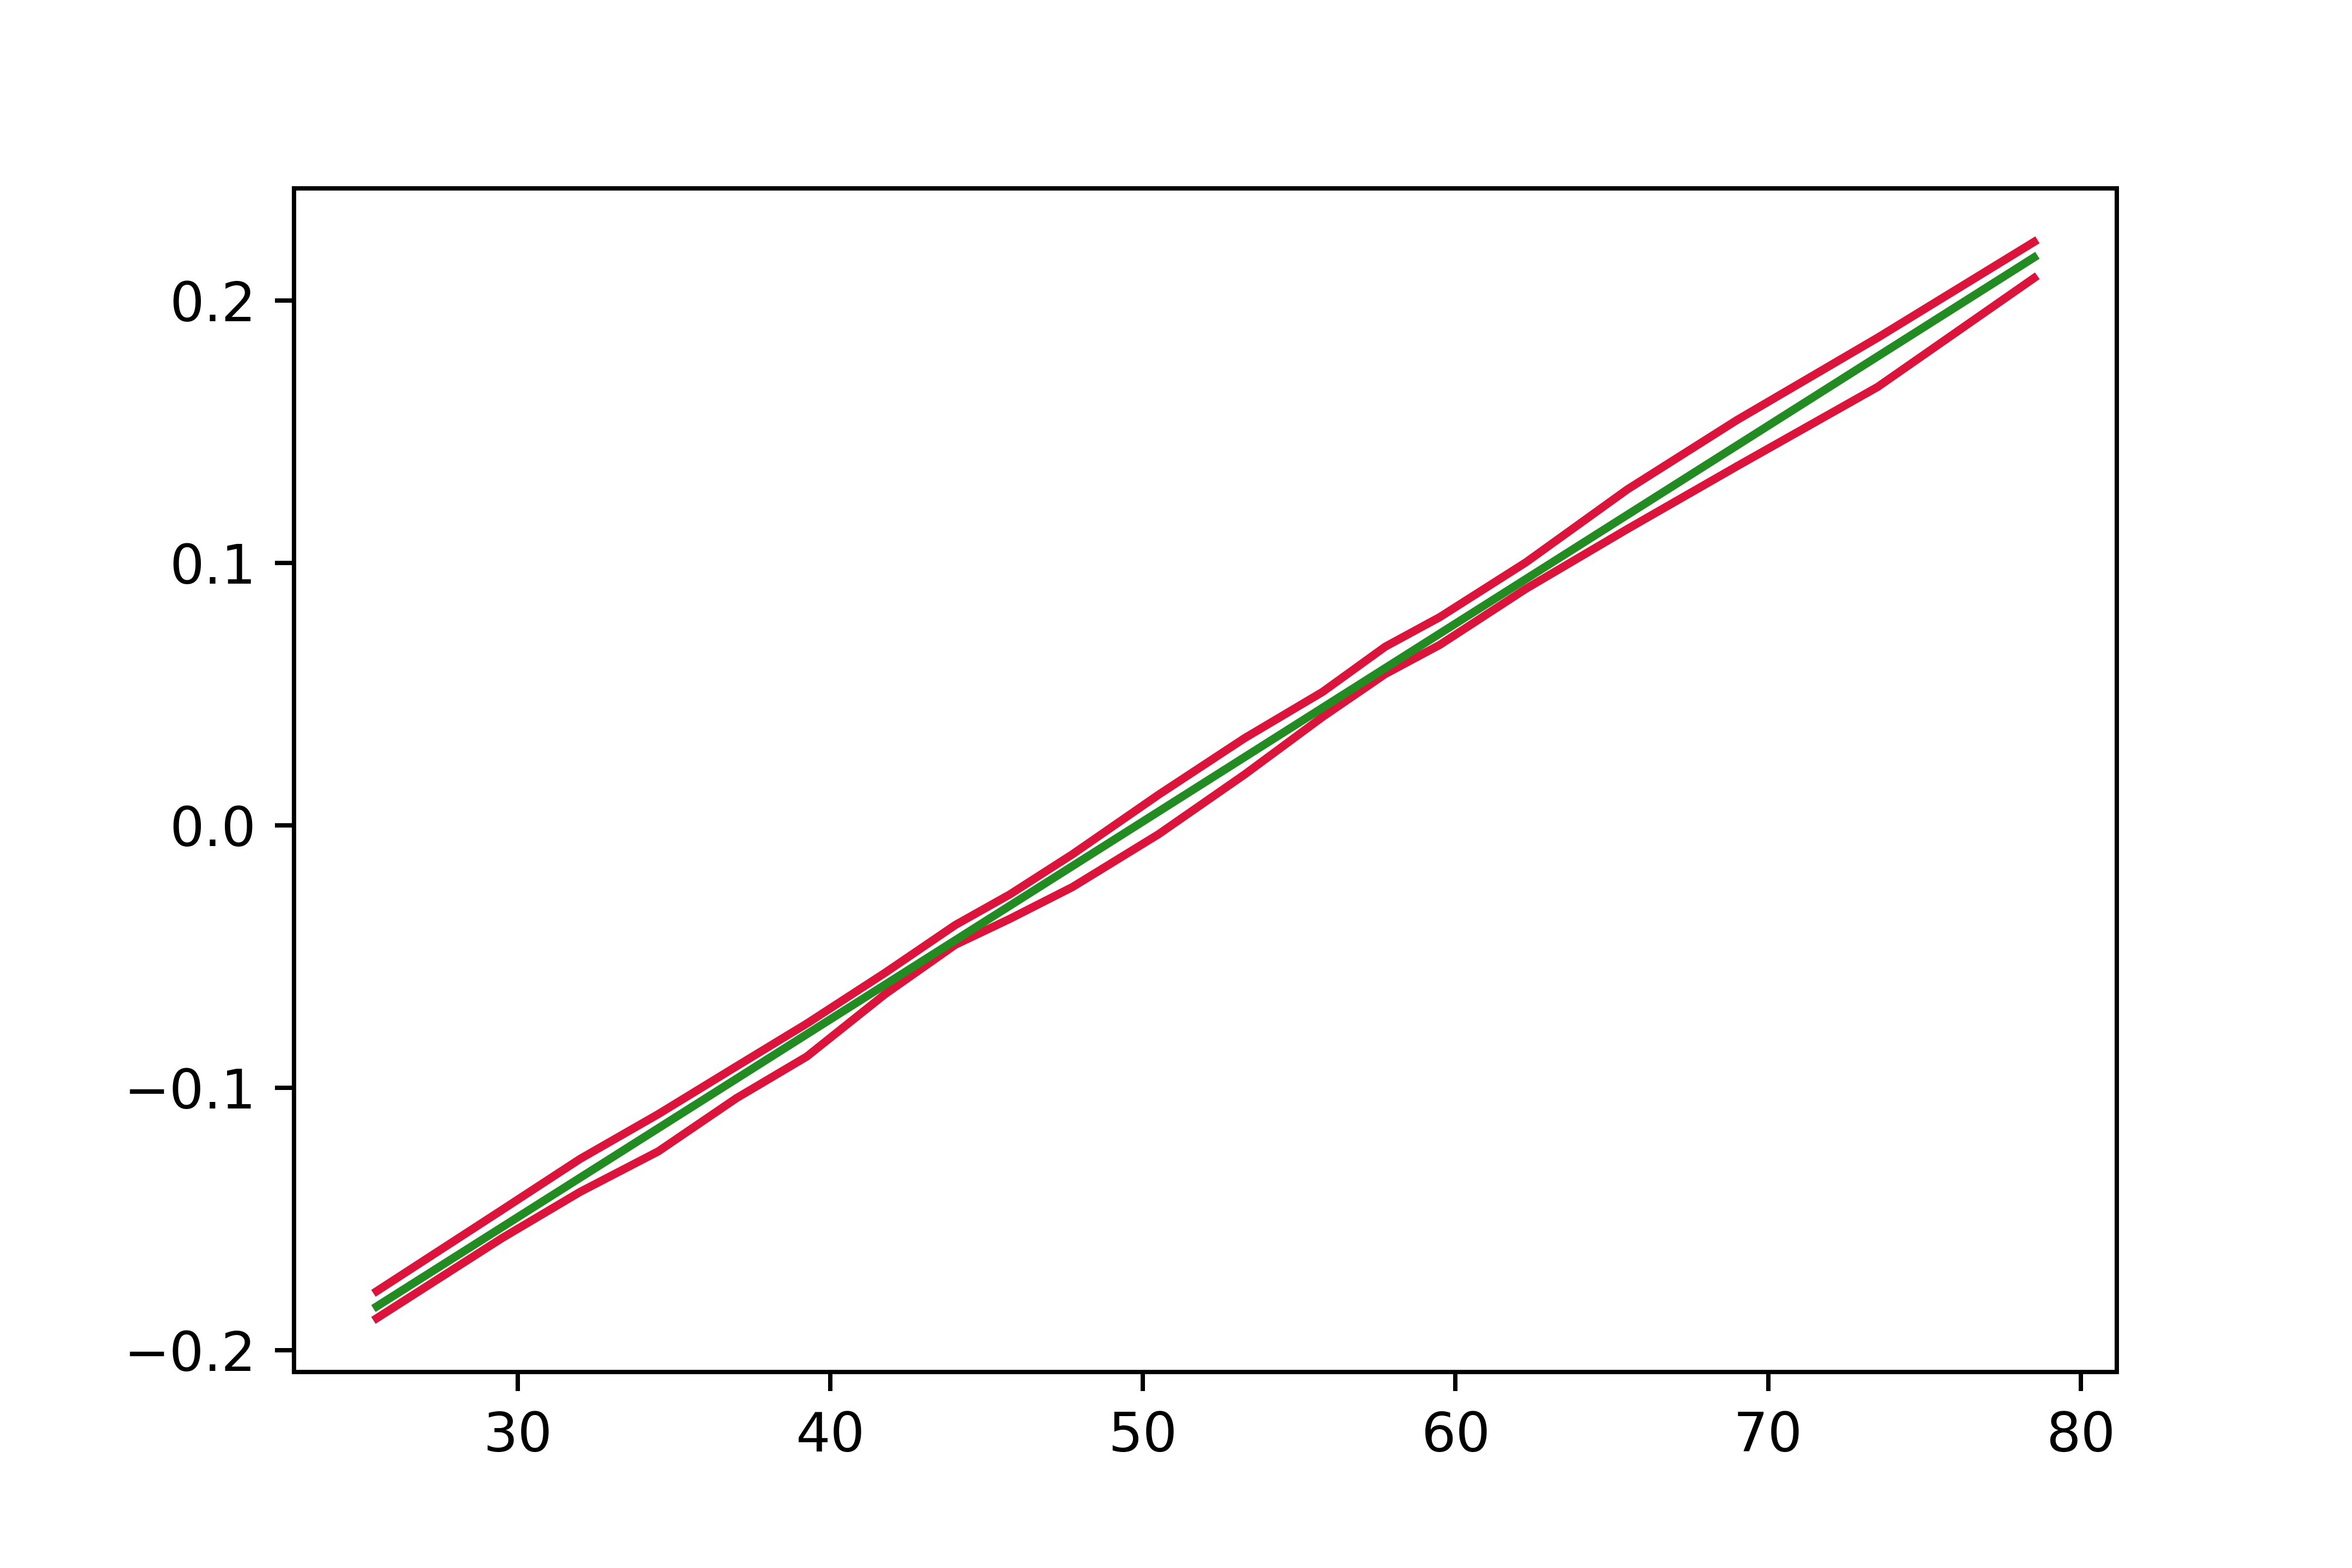
\includegraphics[width=\textwidth]{figures/ALE/chNDexp/spec1_linear_AGE.png}
        \caption{Spec 1 - linear}
    \end{subfigure}%
    \begin{subfigure}{0.5\textwidth}
        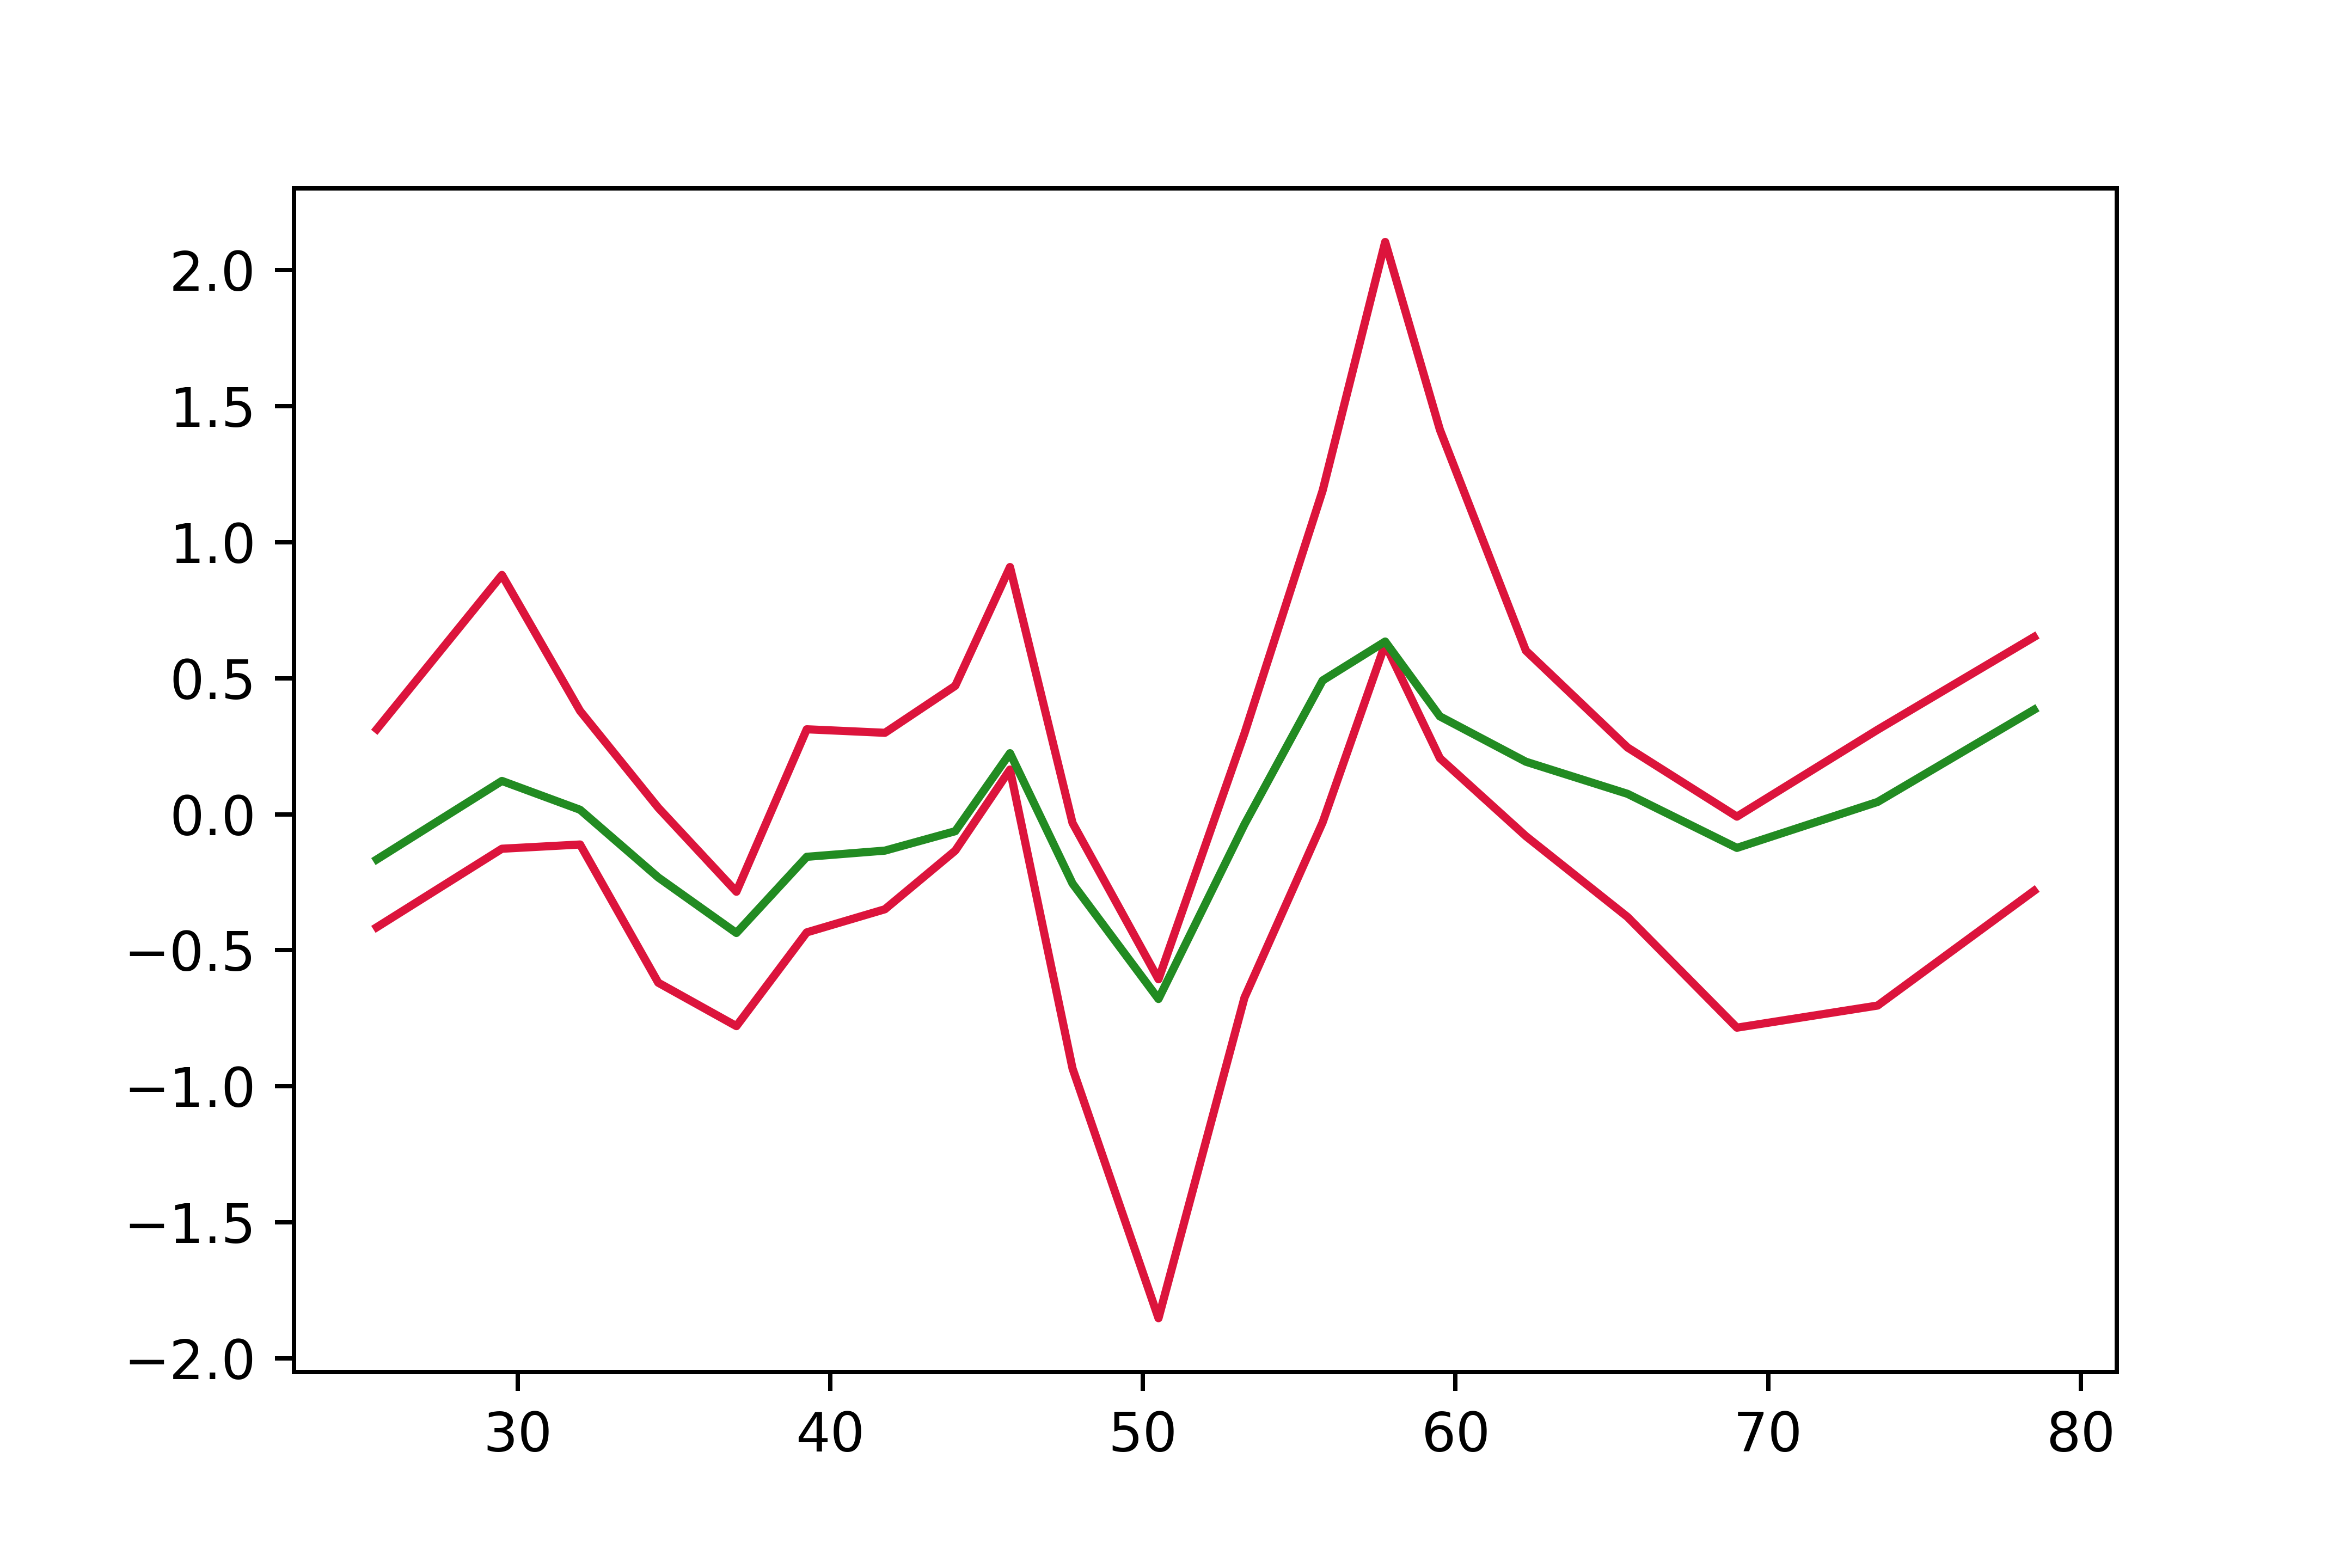
\includegraphics[width=\textwidth]{figures/ALE/chNDexp/spec1_cf_AGE.png}
        \caption{Spec 1 - causal forest}
    \end{subfigure}

    % \begin{subfigure}{0.33\linewidth}
    %     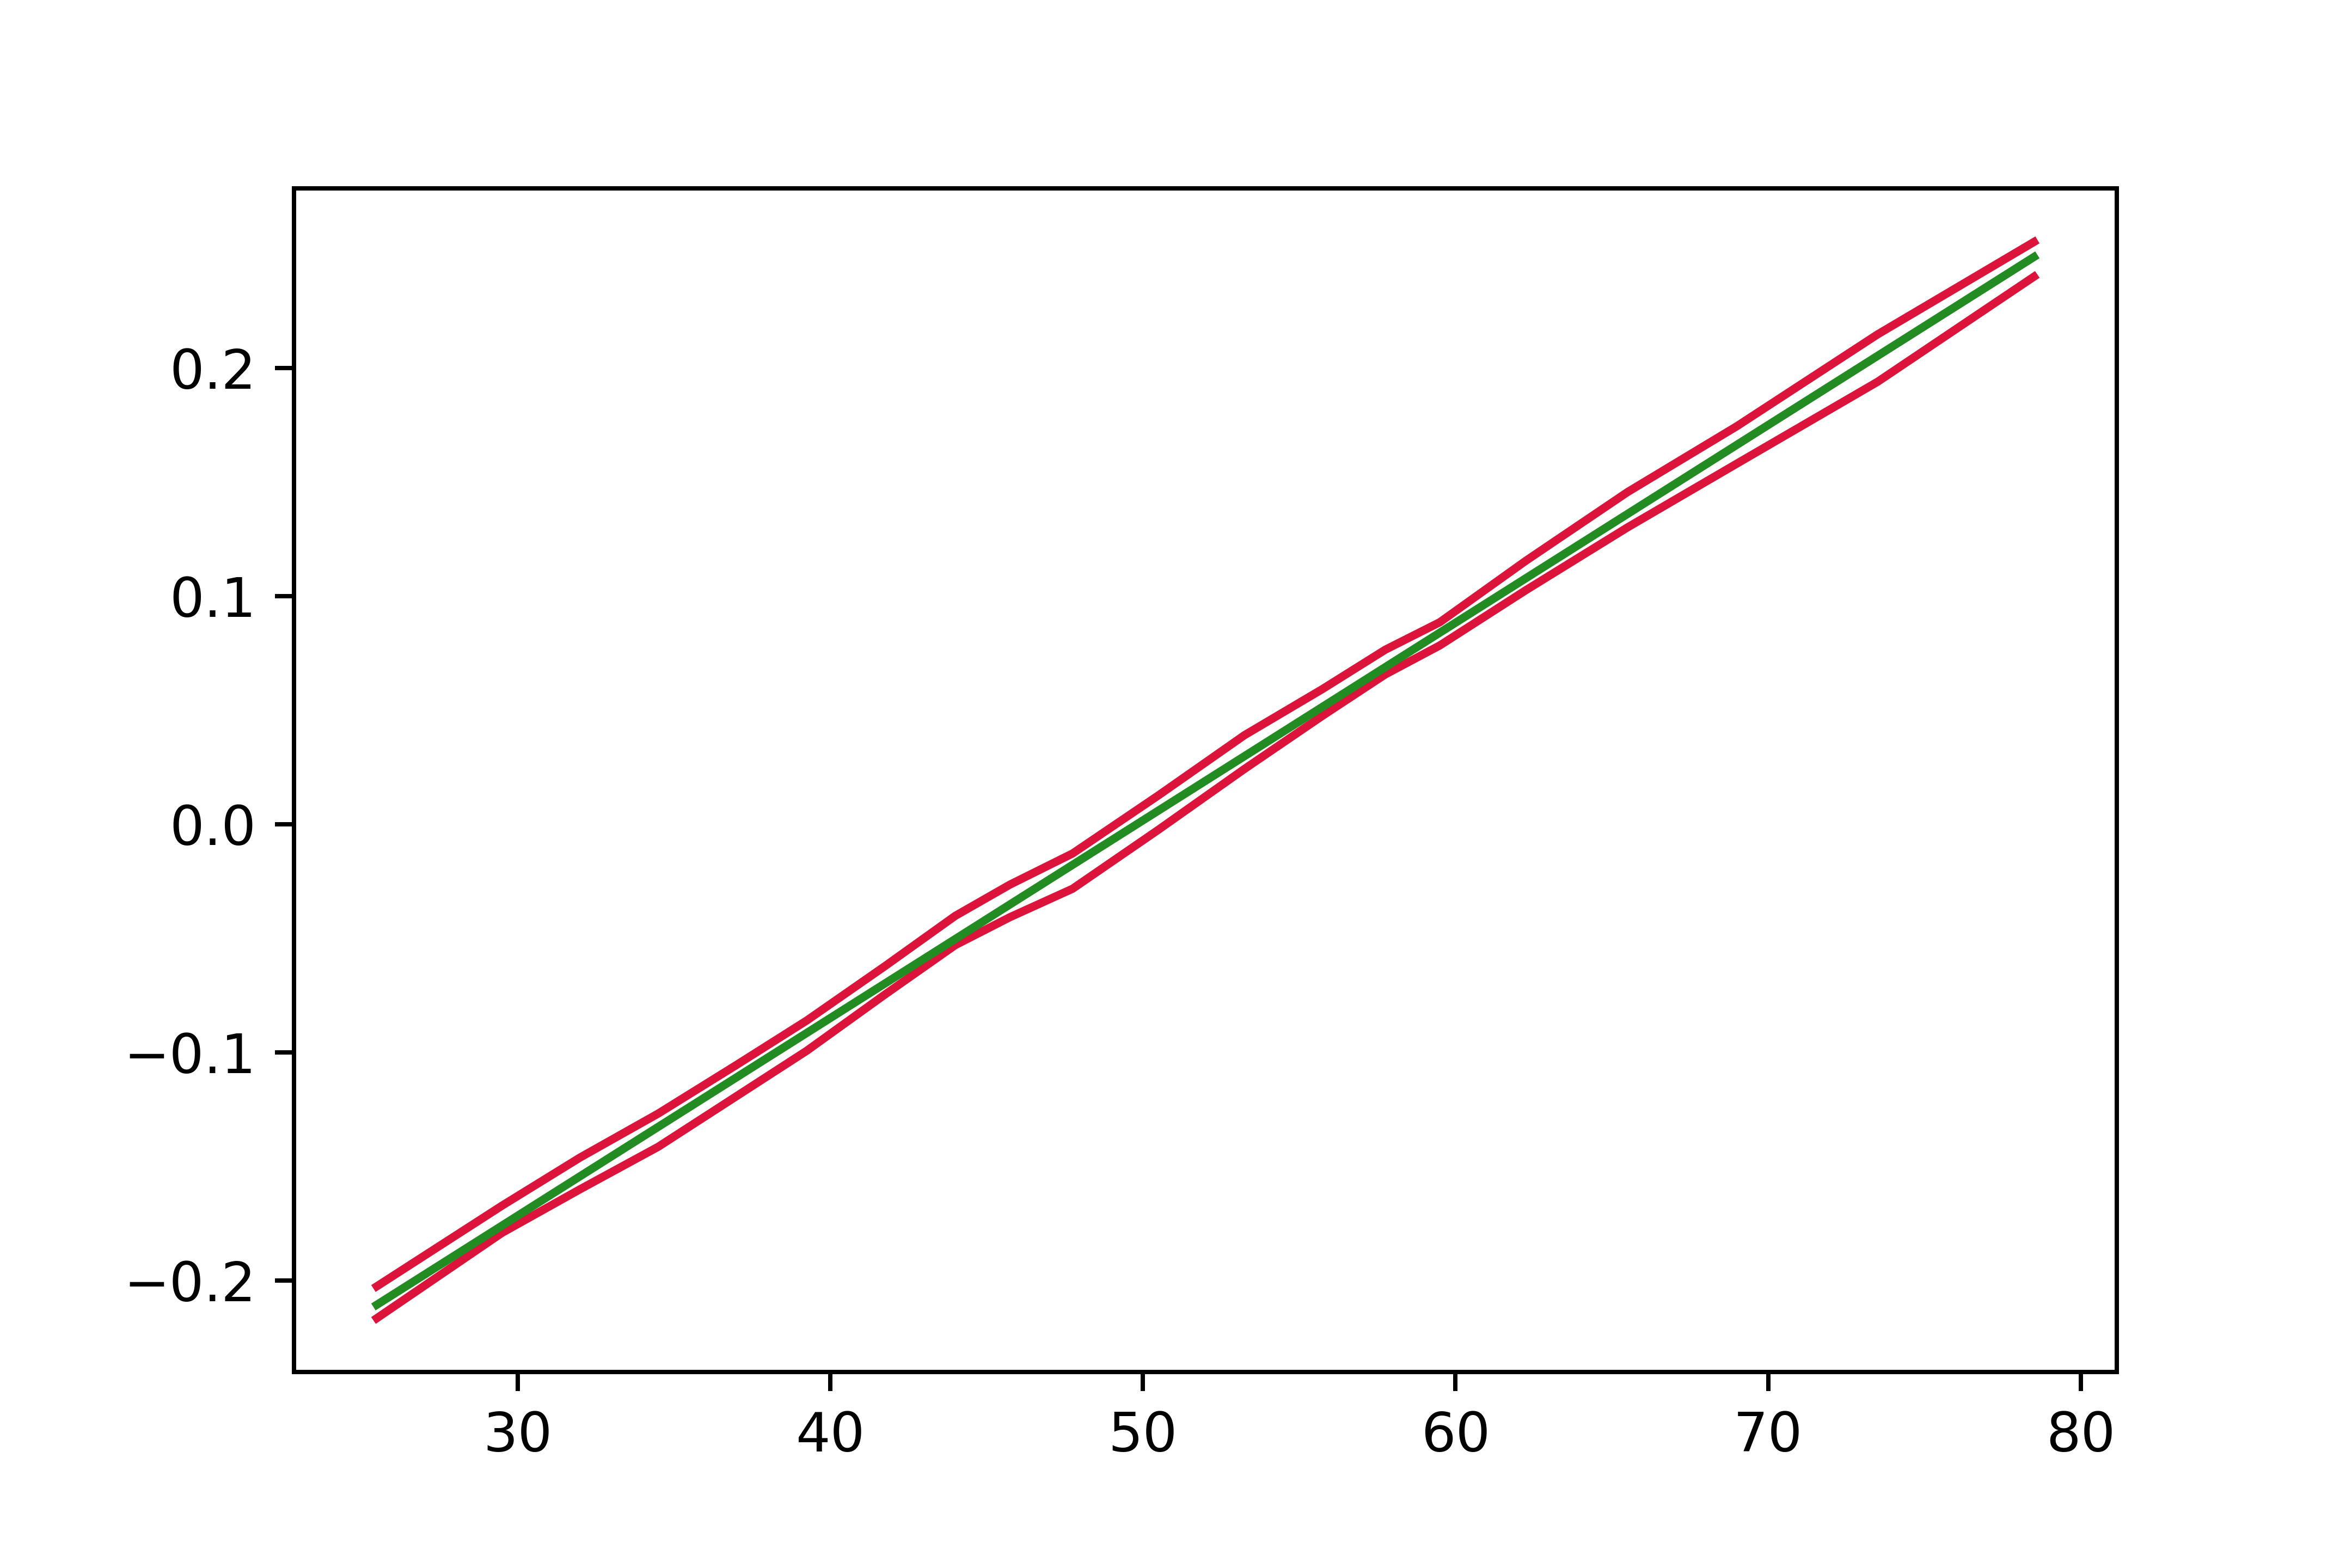
\includegraphics[width=\linewidth]{figures/ALE/chNDexp/spec2_linear_AGE.png}
    %     \caption{Spec 2 - linear}
    % \end{subfigure}\hfill
    % \begin{subfigure}{0.33\linewidth}
    %     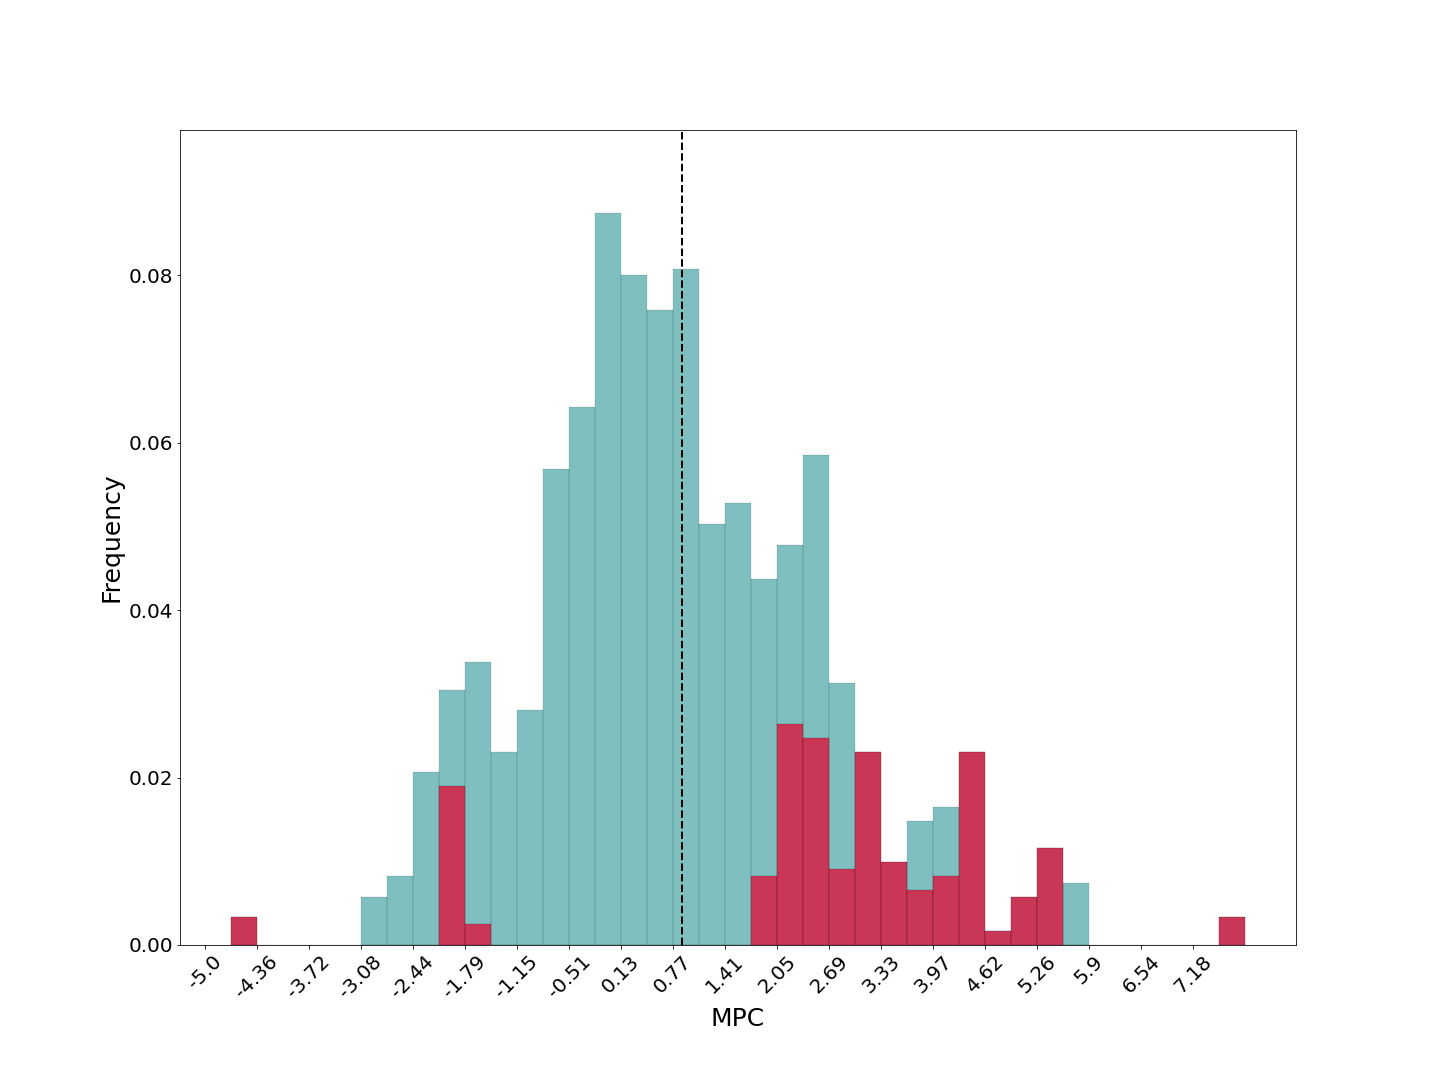
\includegraphics[width=\linewidth]{figures/distributions/spec2_cf_chTOTexp.png}
    %     \caption{Spec 2 - causal forest }
    % \end{subfigure}\hfill
    
    \begin{subfigure}{0.5\linewidth}
        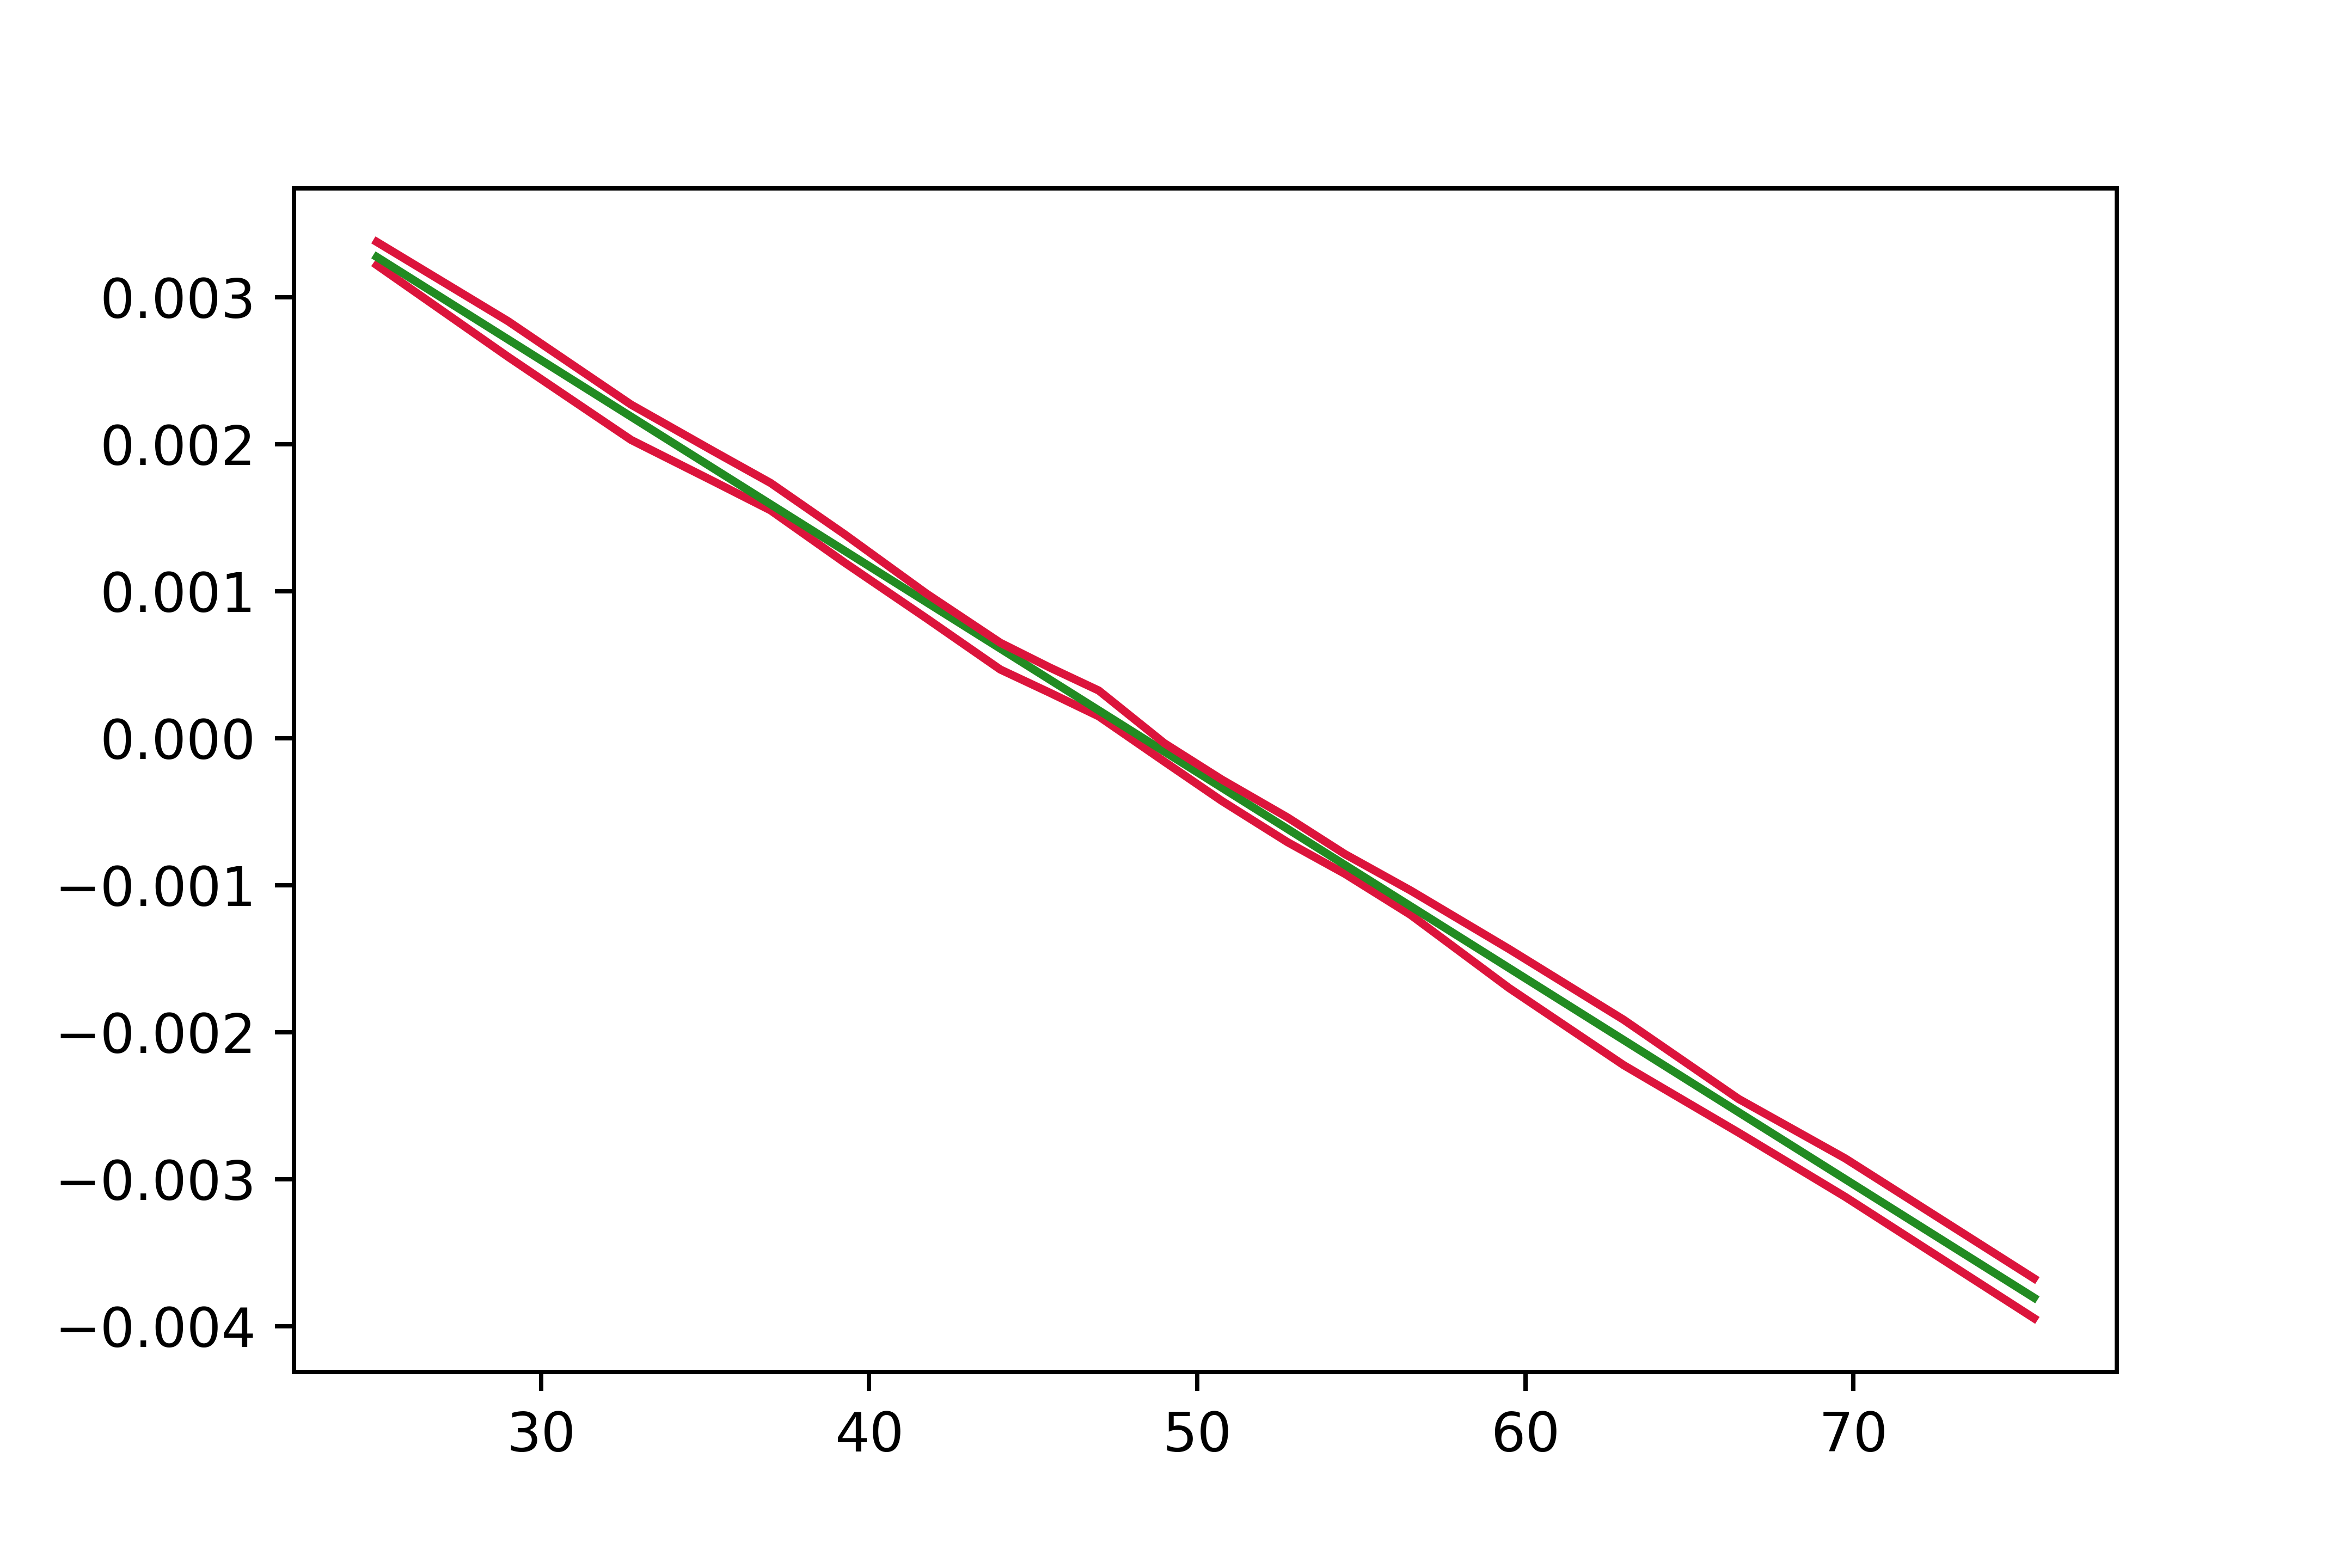
\includegraphics[width=\textwidth]{figures/ALE/chNDexp/spec3_linear_AGE.png}
        \caption{Spec 3 - linear}
    \end{subfigure}%
    \begin{subfigure}{0.5\linewidth}
        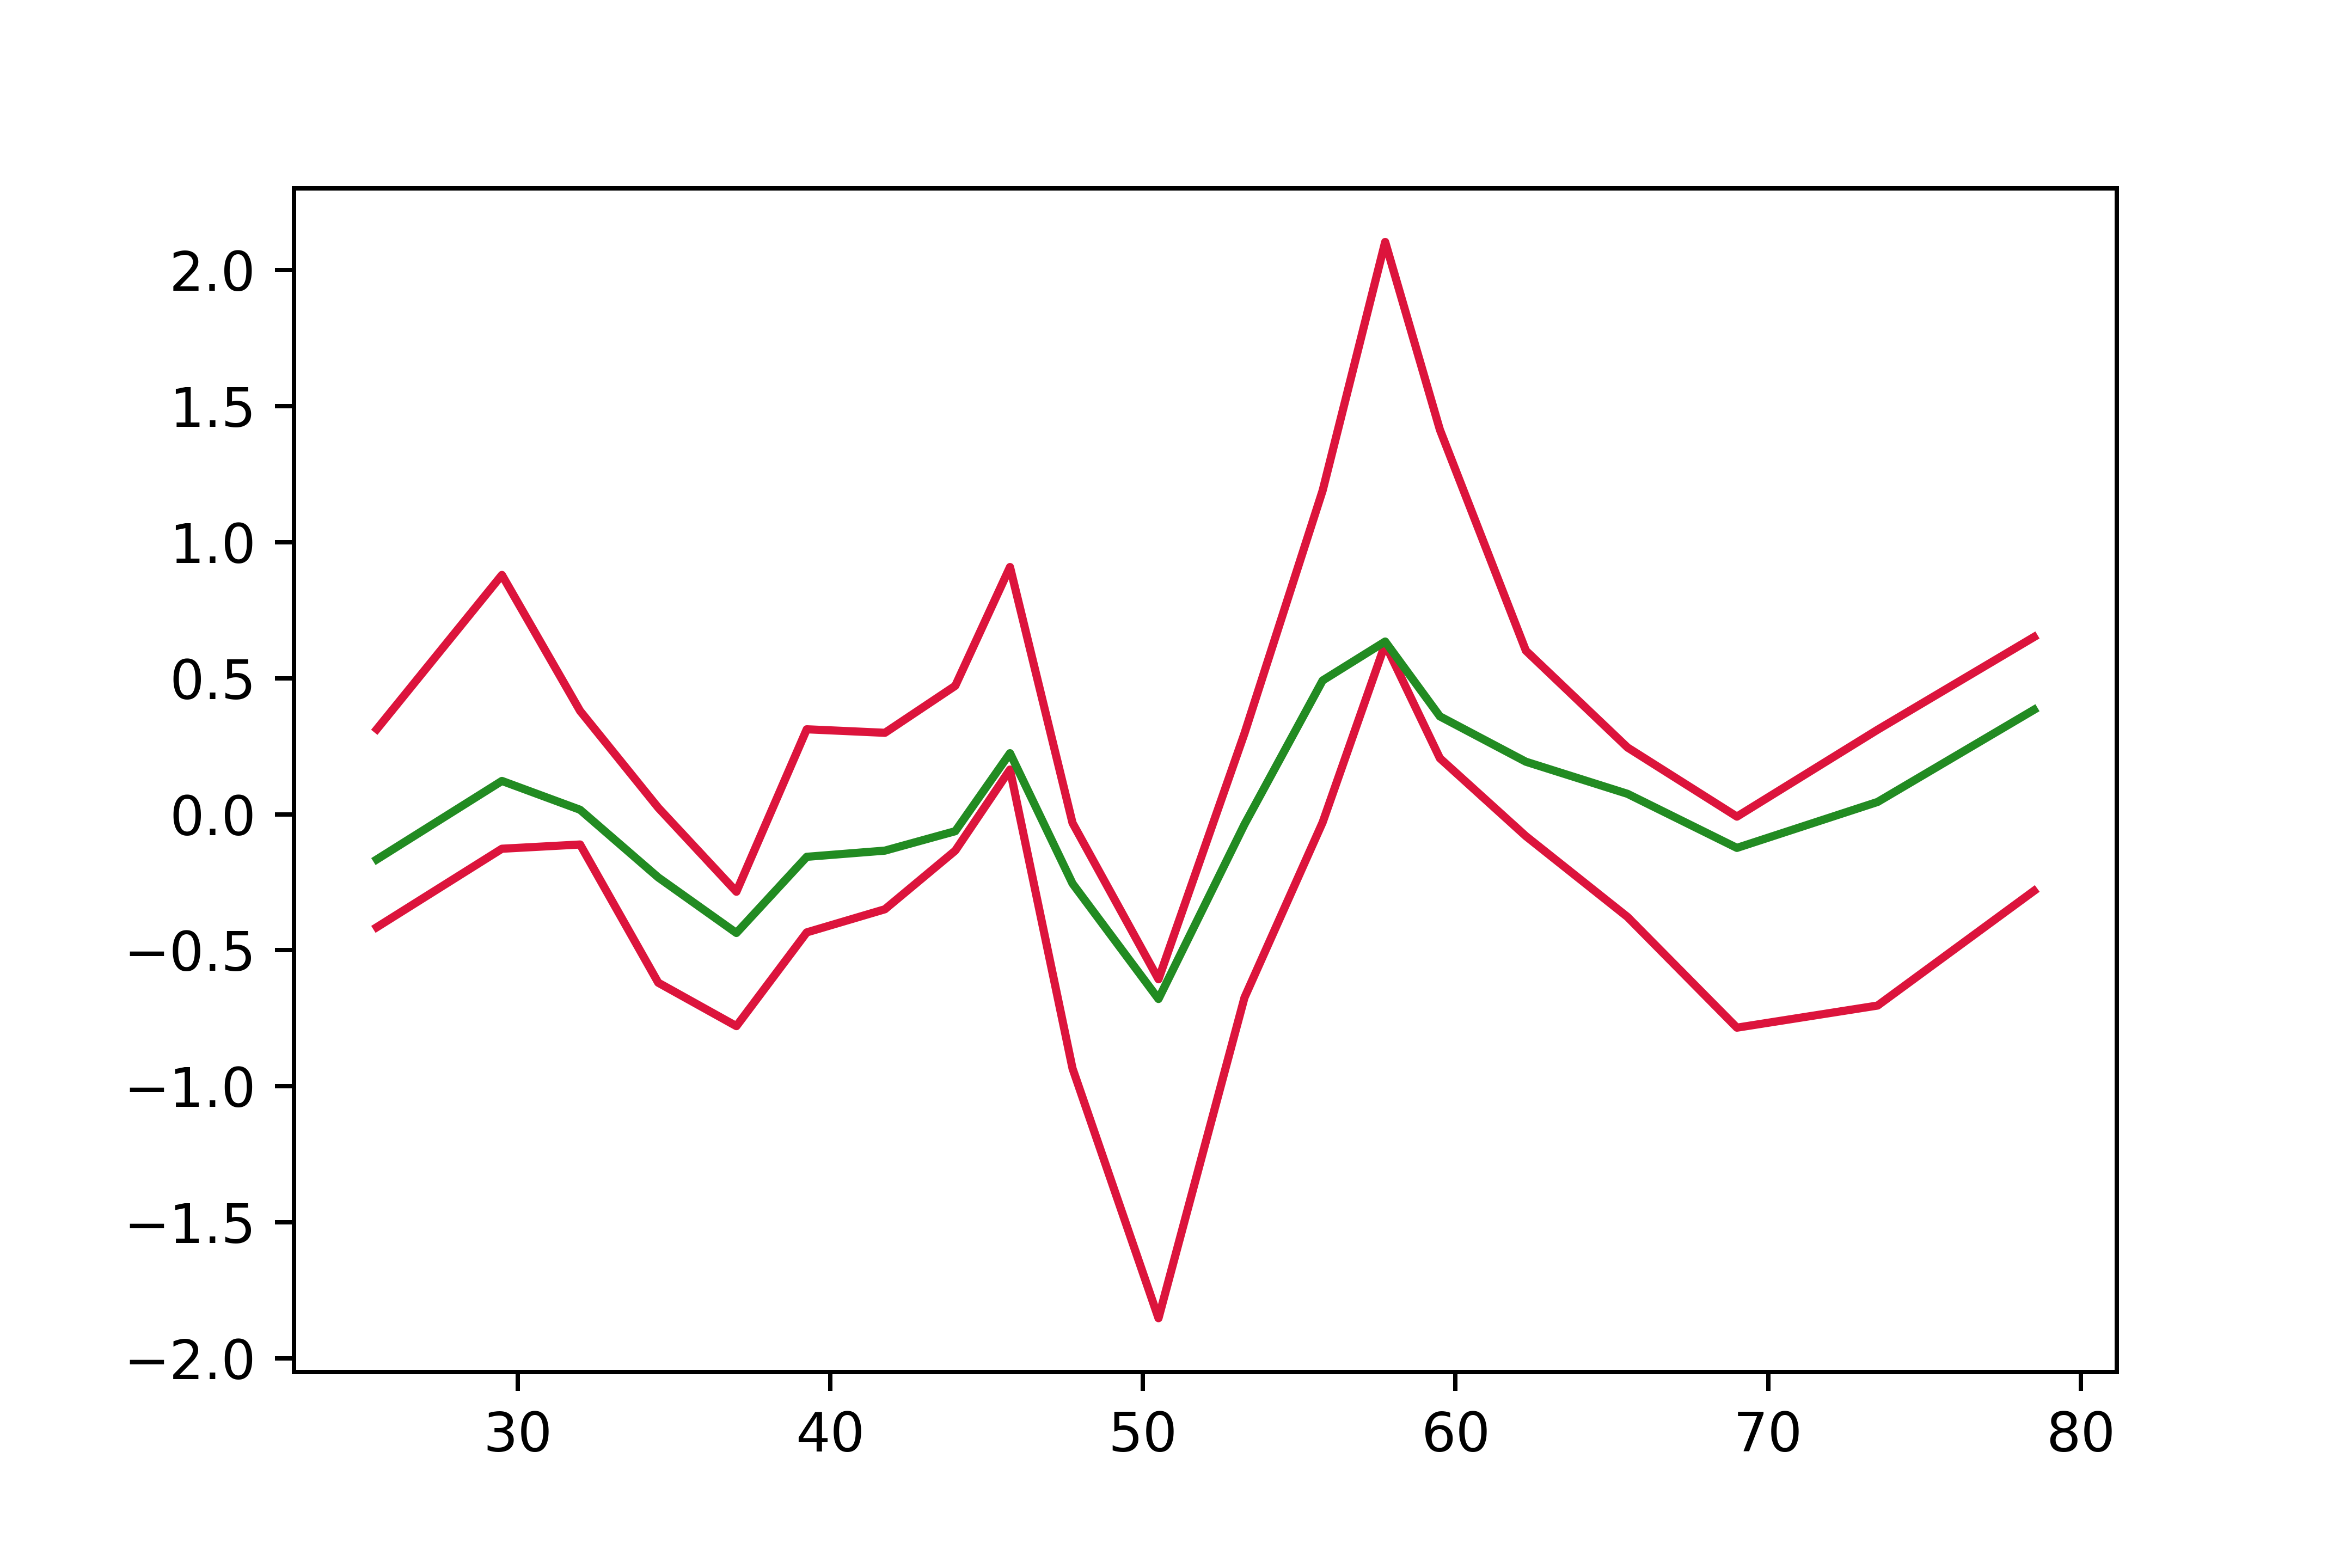
\includegraphics[width=\textwidth]{figures/ALE/chNDexp/spec1_cf_AGE.png}
        \caption{Spec 3 - causal forest}
    \end{subfigure}
    \caption{ALE of Age - non-durable expenditures}
    \label{fig:ale_age}
    % \fnotewide{Red lines show bootstrapped confidence intervals, green lines point estimates of the ALE.}
\end{figure}
Comparing the ALE of the causal forest estimator to the linear model helps us understand where non-linearities play an important role in understanding MPC heterogeneity. We have established in Section \ref{subsec:main_res} that the causal forest estimator reveals more significant MPCs in specification 3, where we control for liquidity, which is likely to occur because of nonlinearities not picked up in the linear CATE model. This notion becomes evident right away when we compare the ALE with respect to age of the linear CATE and the non-linear CATE we retrieve with the causal forest estimator in Figure \ref{fig:ale_age}. The clear positive relationship between age and MPC we find in the linear estimator immediately breaks down in the causal forest based model. Instead, we see a rather unstable relationship with wider pseudo confidence bands. Younger and middle-aged households (45 to 55) seem to be experiencing lower MPCs than older households. However, only for very narrow settings do our bootstrapped CIs completely lie below zero. This signals a very unstable relationship between age and the MPC overall, which is a strong contrast to the linear DML results. These dynamics are observed throughout all consumption categories (see Appendix \ref{app:ale_res}). \\
Interestingly, the role of age in the linear model is reversed once we introduce liquid assets, salary and income in specification 3 (\ref{fig:ale_liquid}). The deviations decrease substantially and the ALE shows that older households seem to have a lower MPC. Given the correlation between age and each of these variables, this underlines their importance since age seems to act as a proxy for them. This bias vanishes by including the \textit{financial status} variables. This dynamic is also upheld in the causal forest estimator, where we see that the effect of age to be more stable and more closely fluctuating around zero. It supports the notion that younger households show a stronger response to the income shock. \\
The main channel identified in the literature is liquidity. Our discussion of the underlying theory of binding borrowing constraints and lacking access to liquid assets provides the intuition for the following analysis. Note that the pattern described here is also present across all consumption categories although the ALE magnitude is varying. The picture painted by the liquidity channel is only in part supported by our results shown in Figure \ref{fig:ale_liquid}. First, the linear estimator shows a negative relationship between MPC and liquidity only for changes in total consumption. When we turn to non-durables and strictly non-durables, the ALE suggests that households with higher liquidity show a stronger positive reaction to the income shock. While these effects are very small, this still suggests that the liquidity channel does not necessarily act as expected in creating MPC heterogeneity. One possible explanation is that for high liquidity households the tax rebate represents a relatively small income shock. Therefore, they do not depend on it financially, are less informed, and are taken more by surprise. However, this phenomenon is quickly turned around by the causal forest results. These fully support the liquidity channel as we find that low liquidity leads to a high MPC, while once a certain threshold in liquid asset holdings is exceeded the MPC is decreased. Hence, the liquidity channel in cases of anticipated income shocks such as the tax rebate is underlined by the causal forest results. Low liquidity households are not able to react at the announcement to the shock and thus show a strong reaction once the tex rebate is received. On the other hand, a higher level of liquidity enables households to increase consumption before receiving the rebate and smooth consumption level overall. \\
\begin{figure}[t]
    \centering
    \begin{subfigure}{0.5\textwidth}
        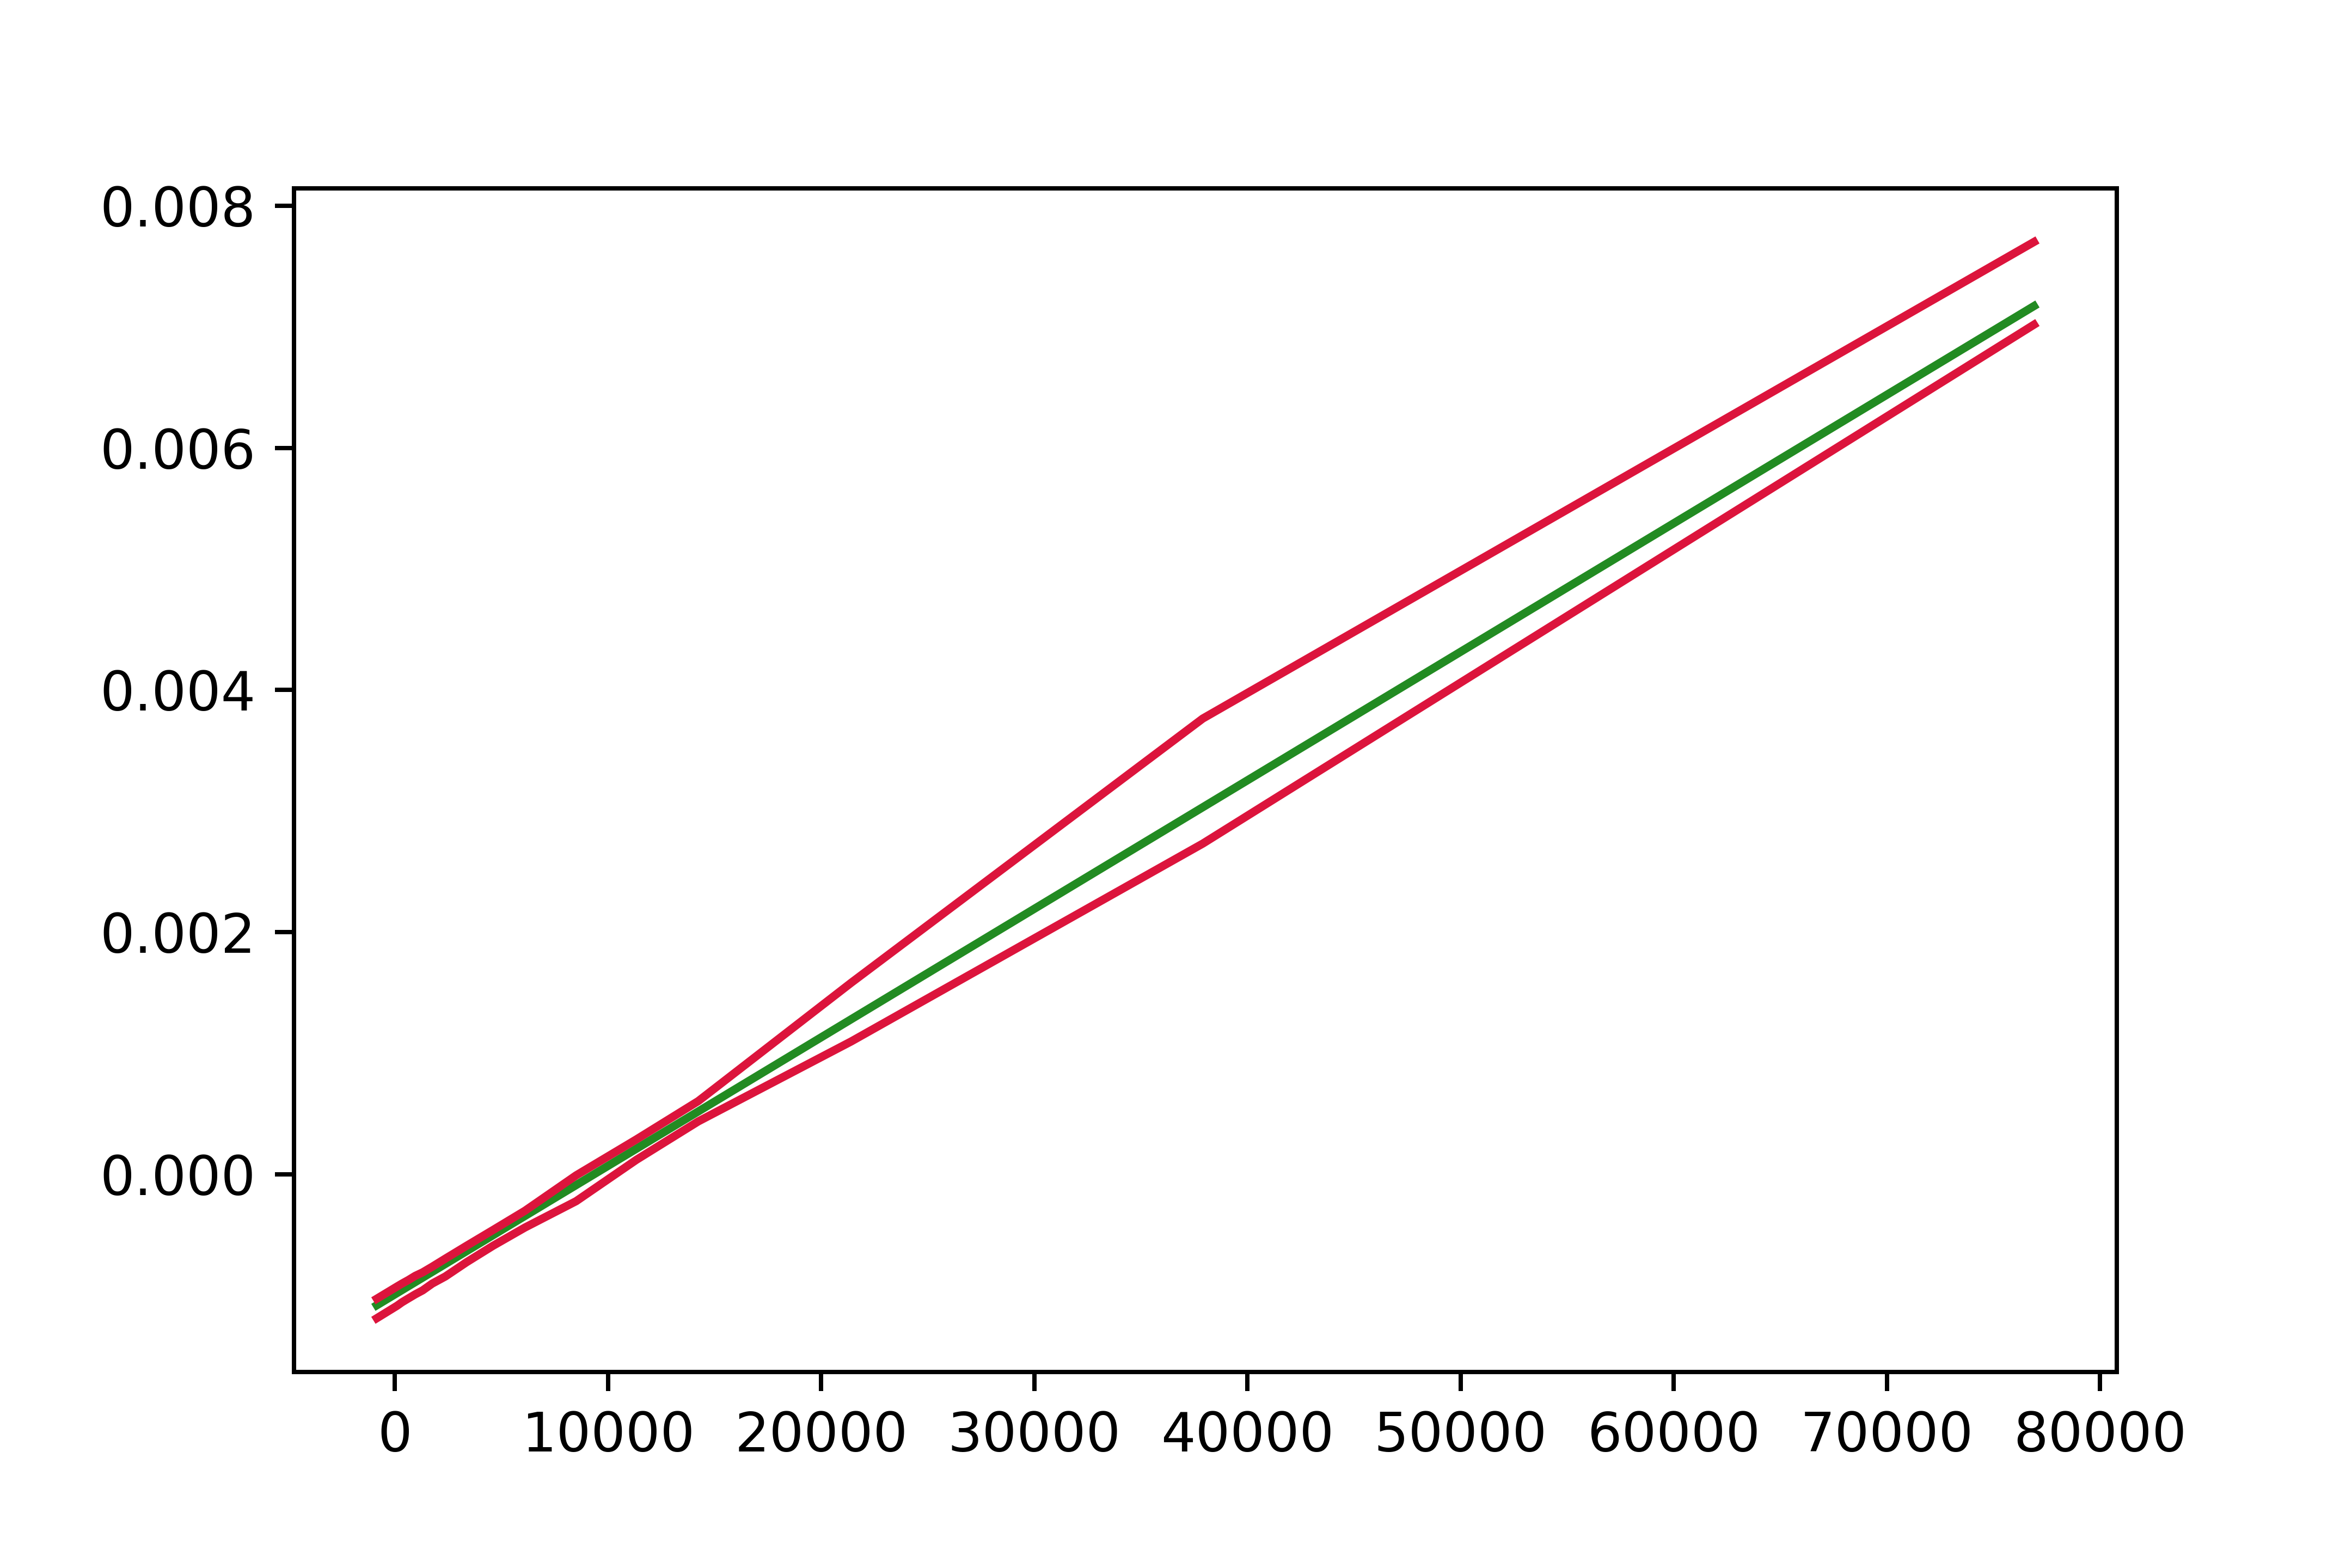
\includegraphics[width=\textwidth]{figures/ALE/chNDexp/spec3_linear_liqassii.png}
        \caption{Spec 3 - linear}
    \end{subfigure}%
    \begin{subfigure}{0.5\textwidth}
        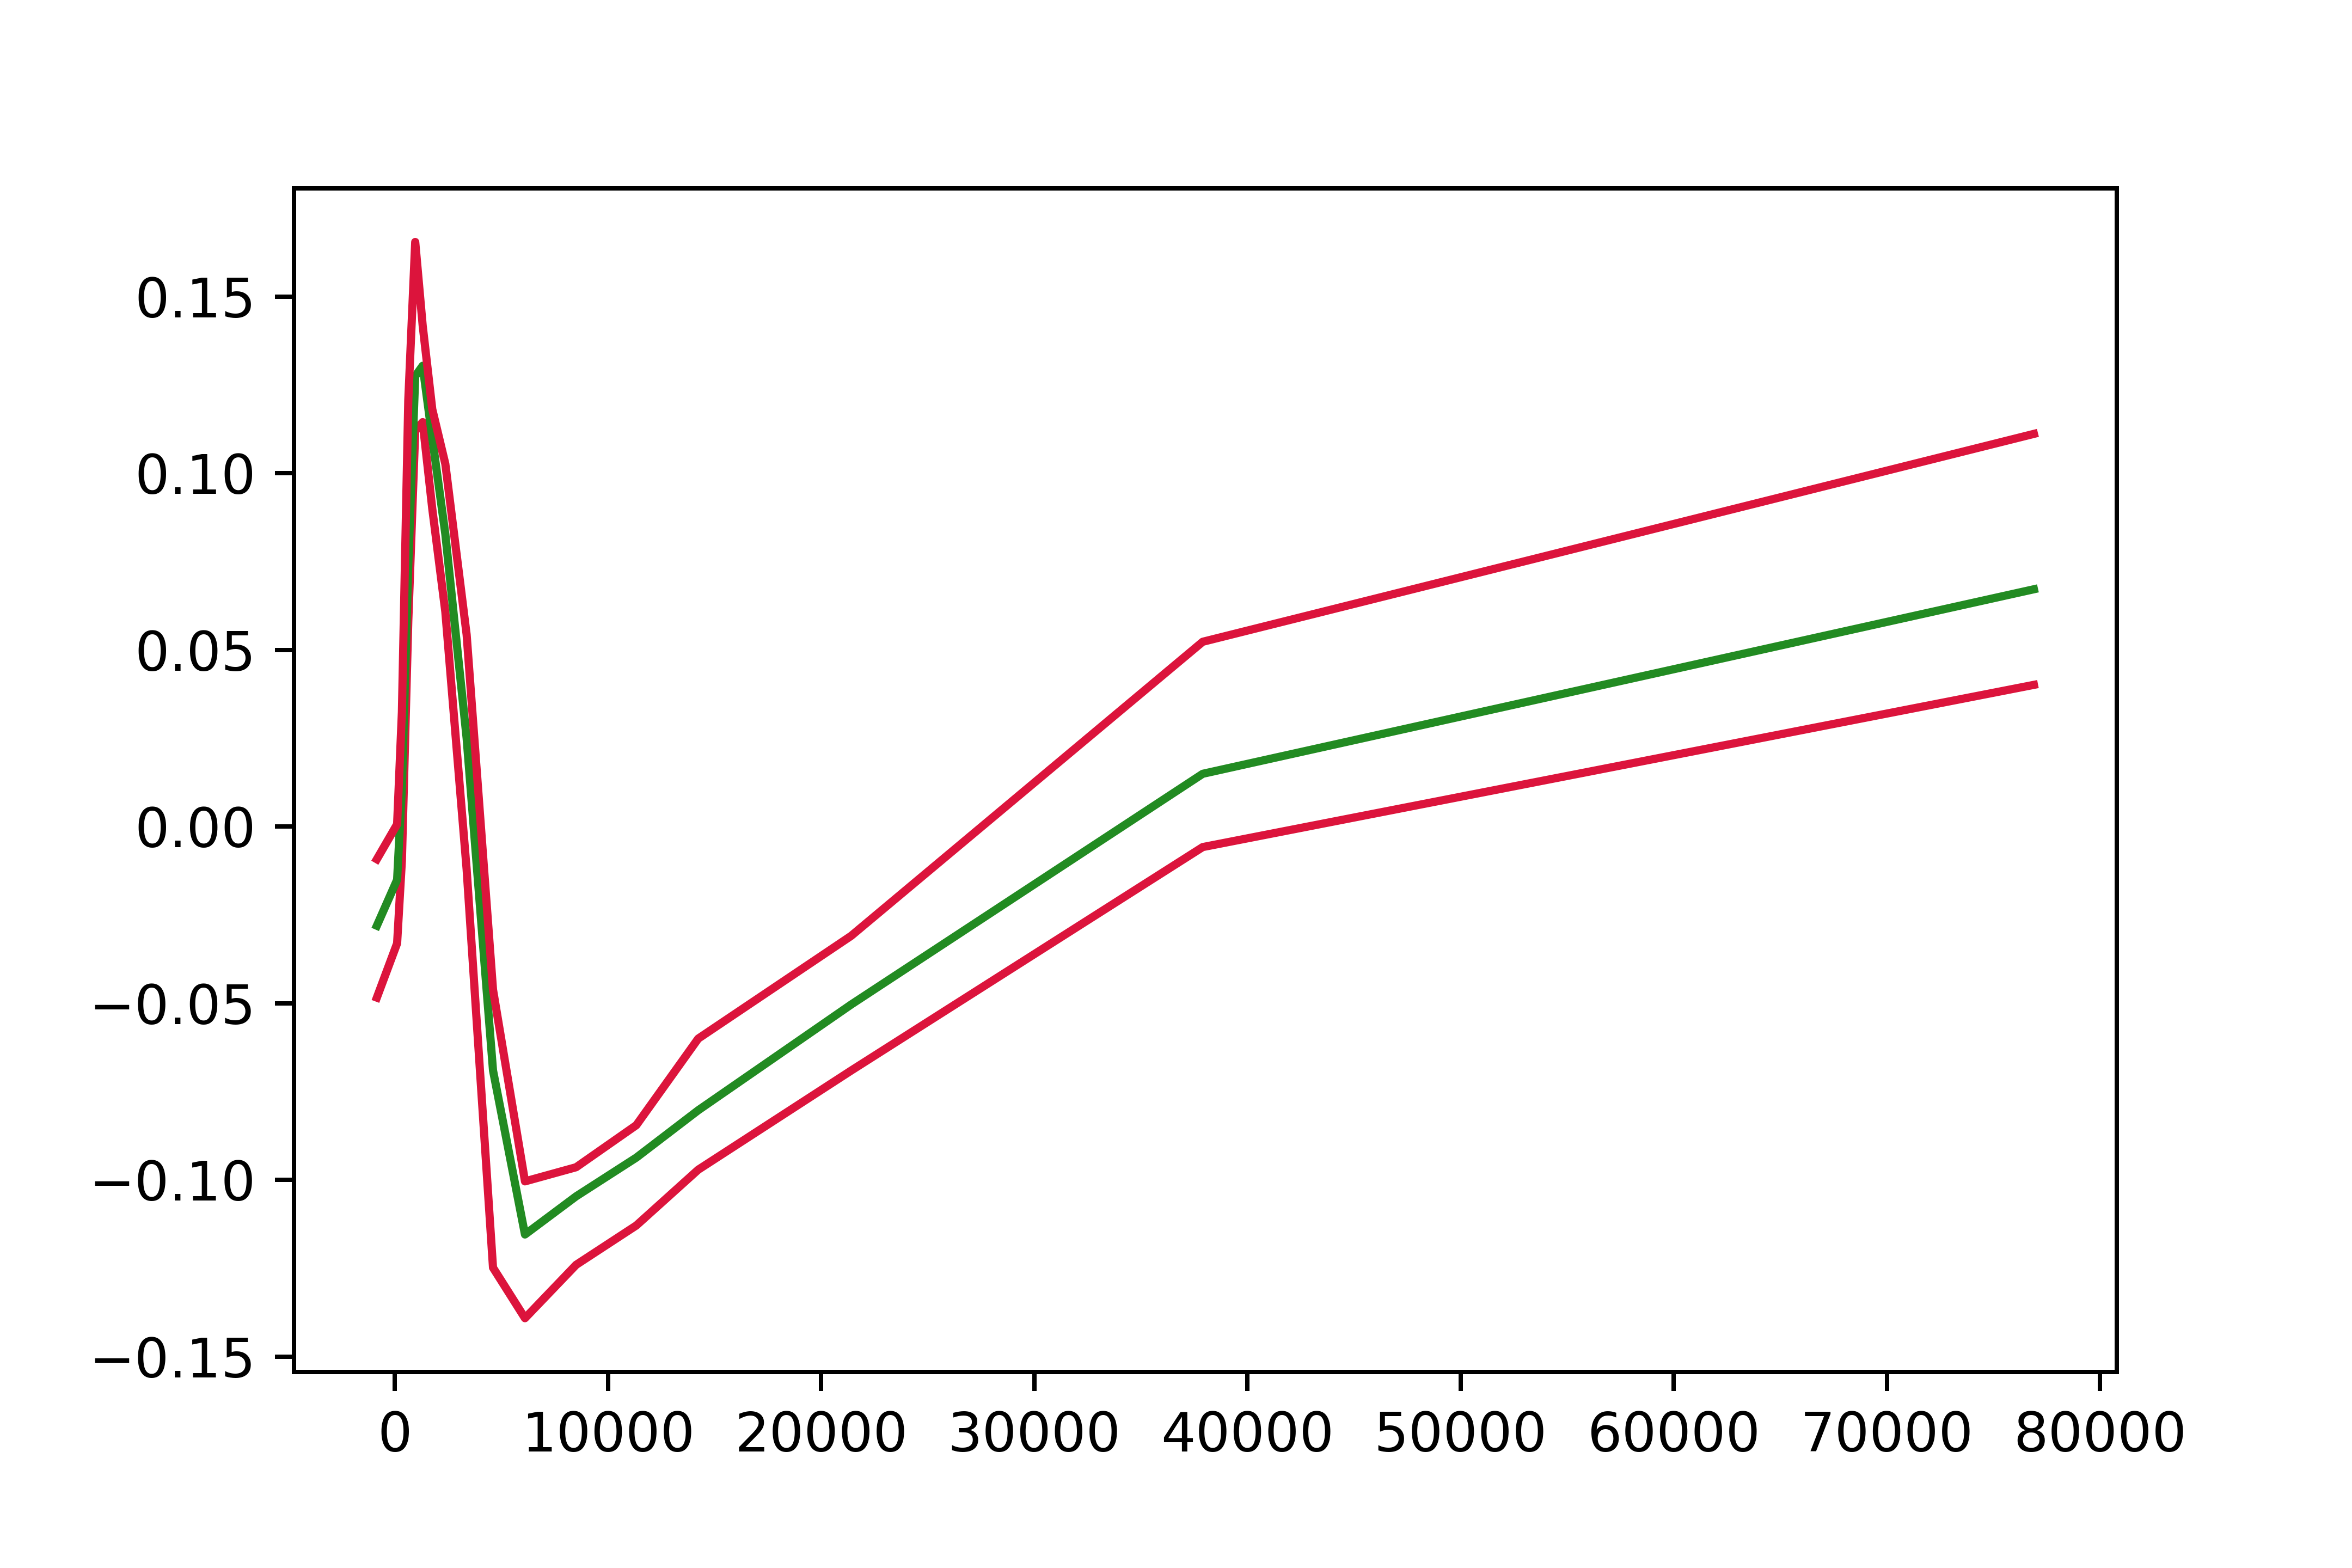
\includegraphics[width=\textwidth]{figures/ALE/chNDexp/spec3_cf_liqassii.png}
        \caption{Spec 3 - causal forest}
    \end{subfigure}
    \caption{ALE of liquid assets - non-durable expenditures}
    \label{fig:ale_liquid}
\end{figure}
Interestingly, the causal forest reveals that at the very bottom of the liquidity distribution, households show a negative response to rebate receipt. These negative responses might explain why the linear DML shows no role of liquidity at low levels of liquidity as it does not fully capture non-linearities and interactions, leaving the estimator biased. On the other hand, they are contrary to the main idea of the liquidity channel. This result shows that the clear relationship the liquidity channel paints in theory is more blurry in the data. Instead, the negative effect of very low levels of liquidity on the predicted MPC highlights a new role. A possible explanation might again be related to the circumstances under which the stimulus is received. Households with no liquidity might save up the stimulus to build up a buffer during the times of economic downturn as were taking place in 2008. \\
On the other hand, the sharp drop after roughly 2,000 USD suggests that households that were capable of increasing their consumption at the announcement by tapping into their liquid assets consequently have a lower MPC out of the rebate as they save it to further smooth consumption by saving it. The drift to a positive role of liquidity once households have high liquid asset holdings is very unstable as evidenced by the very wide CIs that also include negative values and zero across all levels of liquidity. Most likely, this is due to the small number of households in our sample that report such high levels of liquidity leaving the causal forest performing imprecisely. \\
\begin{figure}[t]
    \centering
    \begin{subfigure}{0.5\textwidth}
        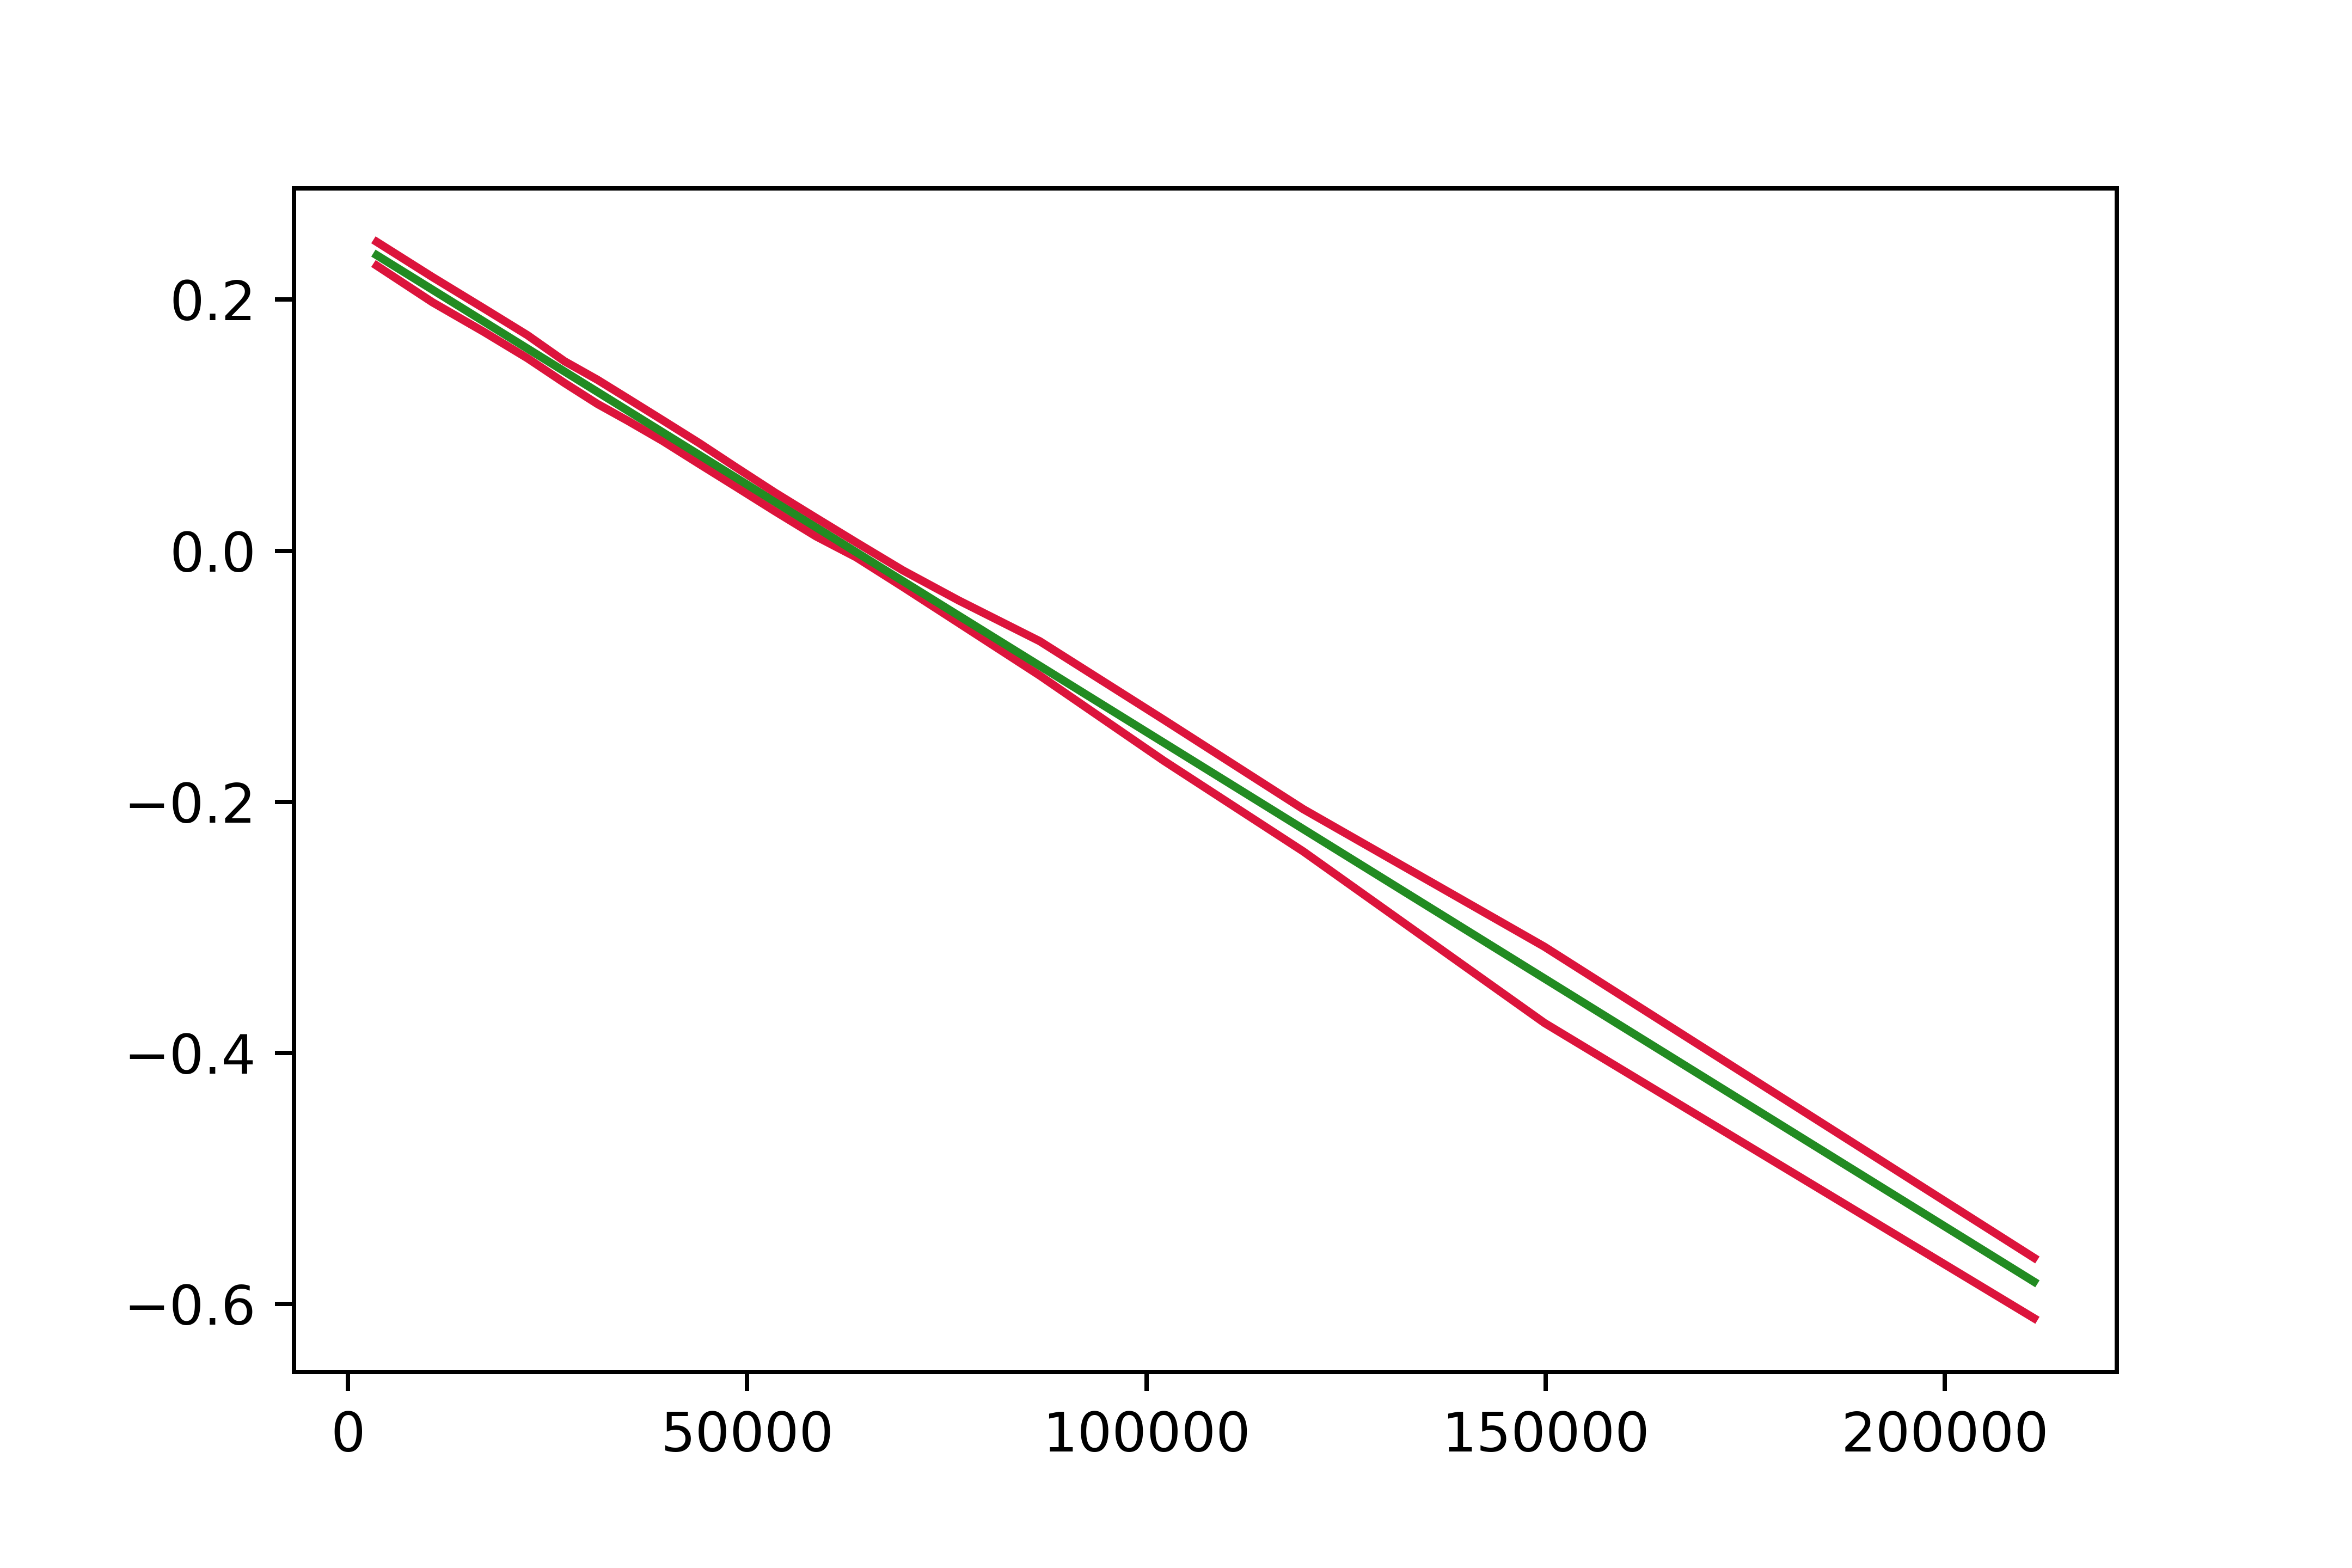
\includegraphics[width=\linewidth]{figures/ALE/chNDexp/spec3_linear_FSALARYM.png}
        \caption{Salary - linear}
    \end{subfigure}\hfill
    \begin{subfigure}{0.5\textwidth}
        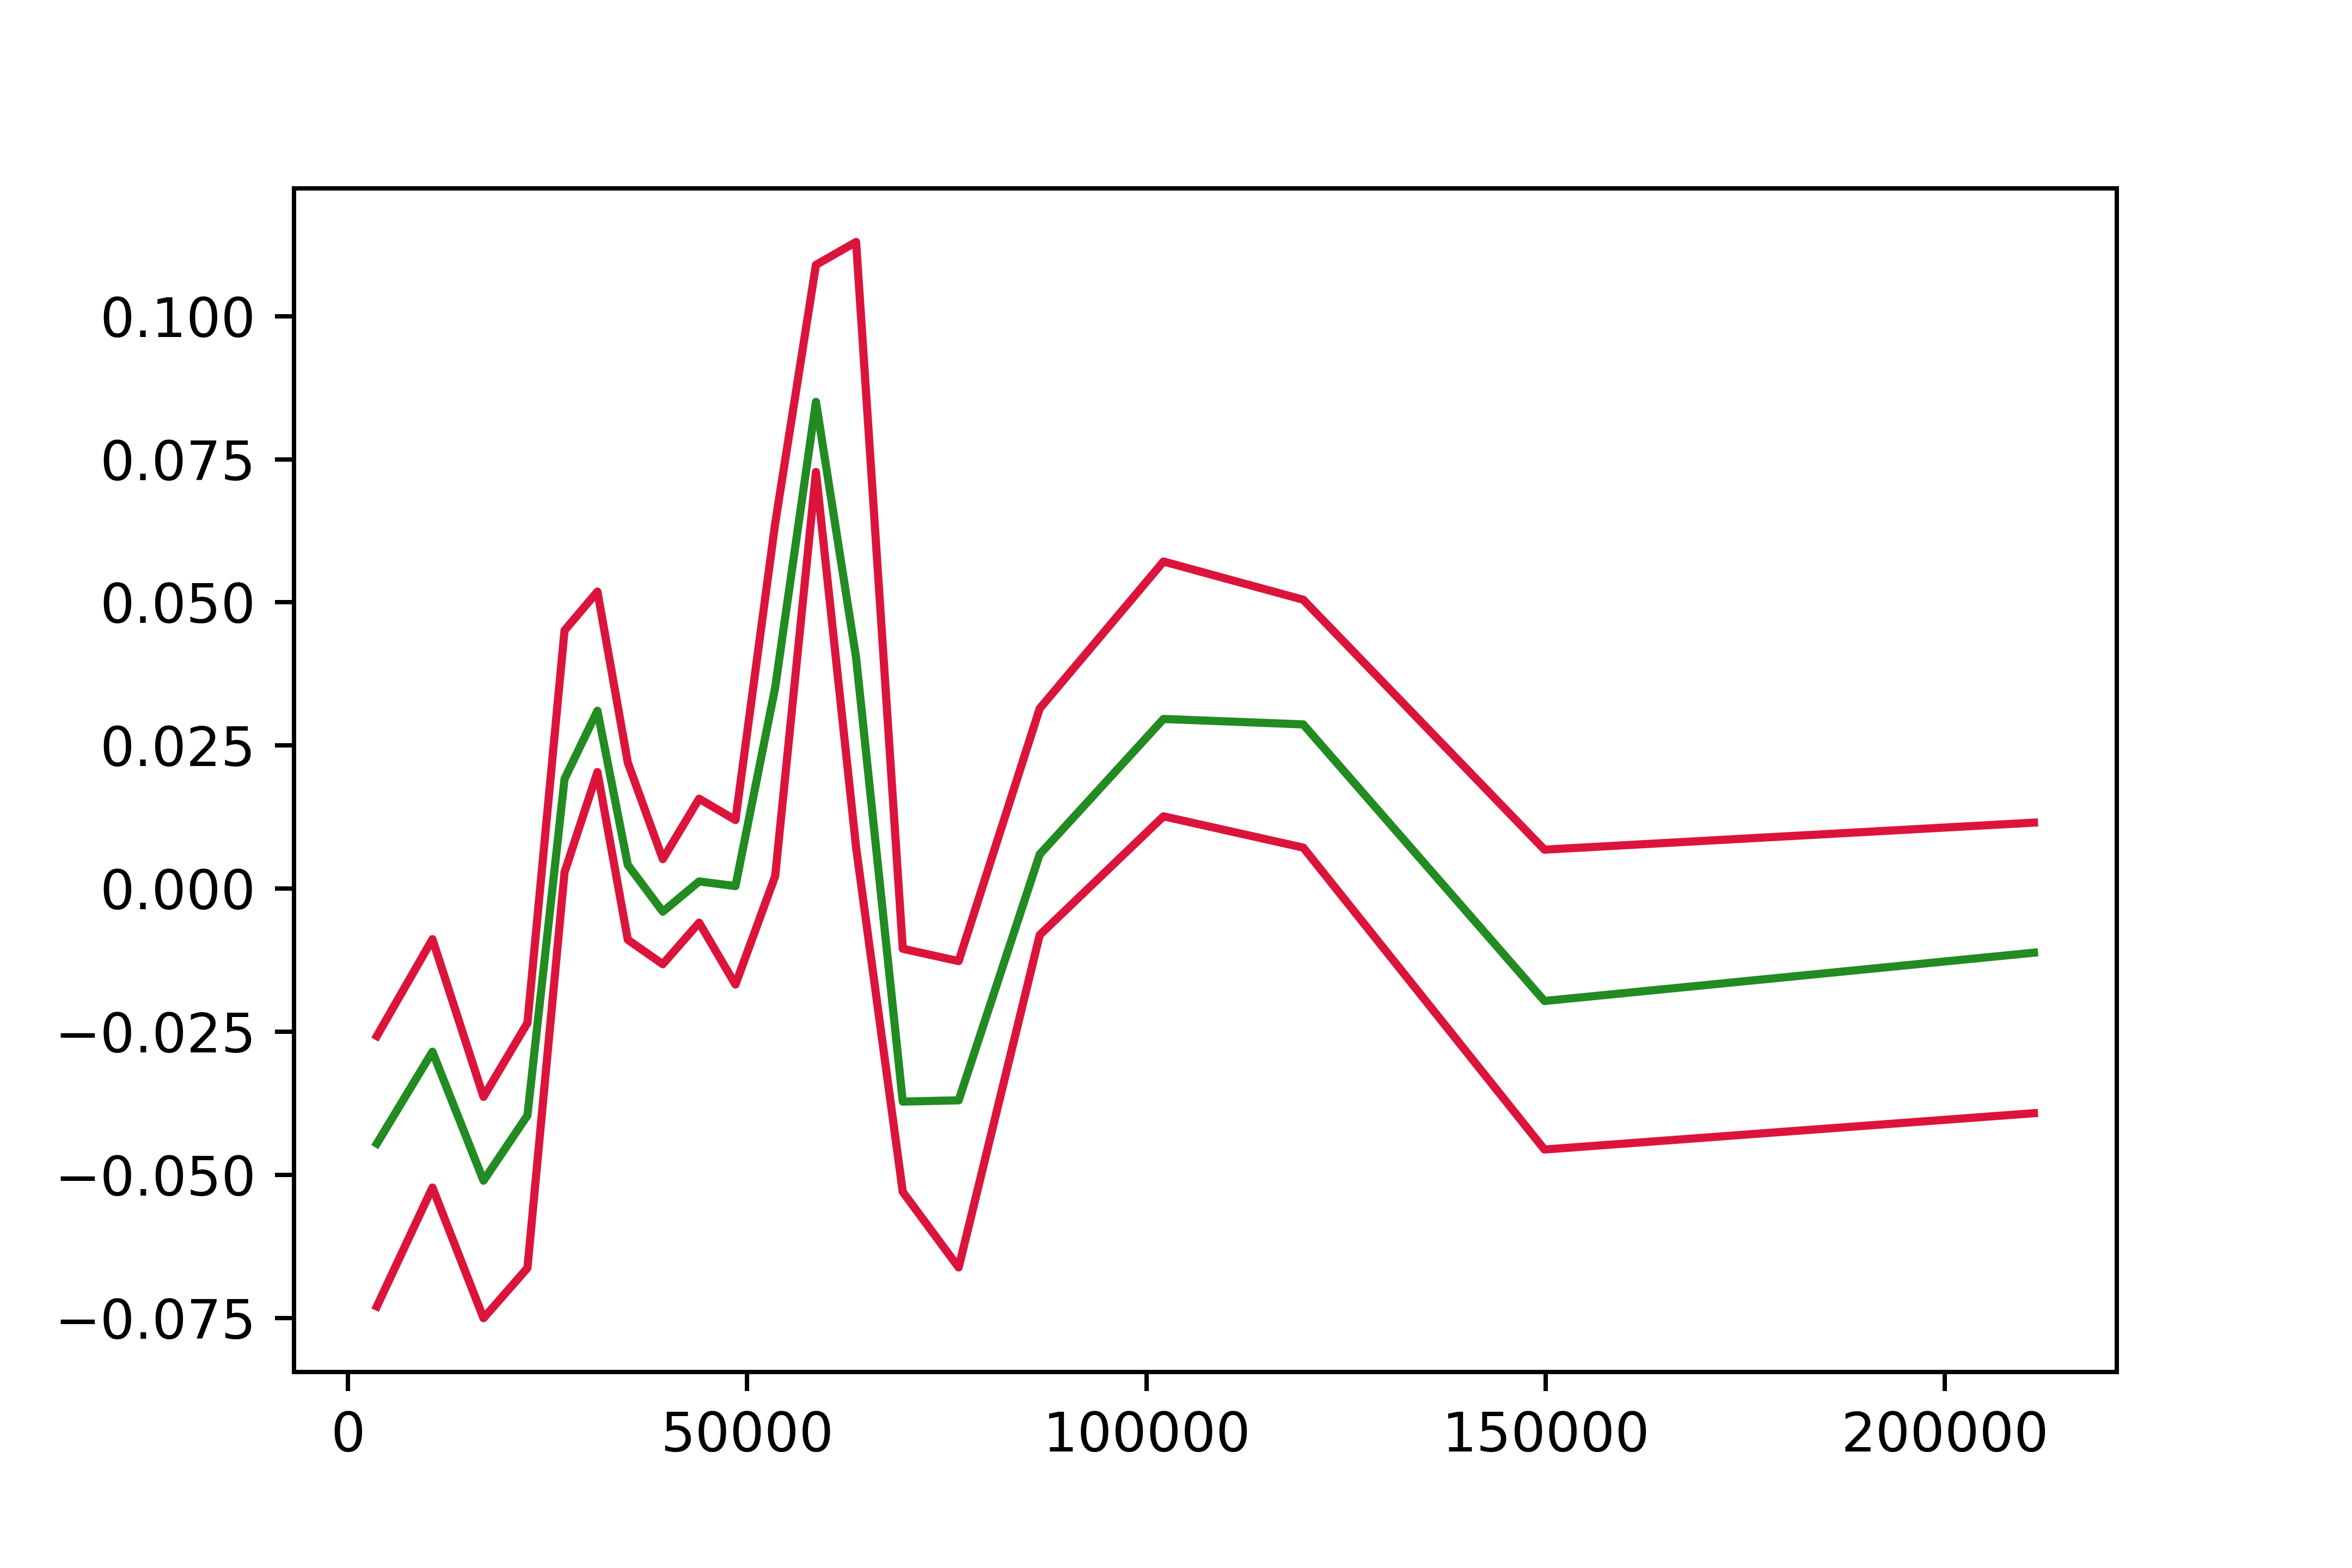
\includegraphics[width=\linewidth]{figures/ALE/chNDexp/spec3_cf_FSALARYM.png}
        \caption{Salary - causal forest}
    \end{subfigure}\hfill

    \begin{subfigure}{0.5\textwidth}
        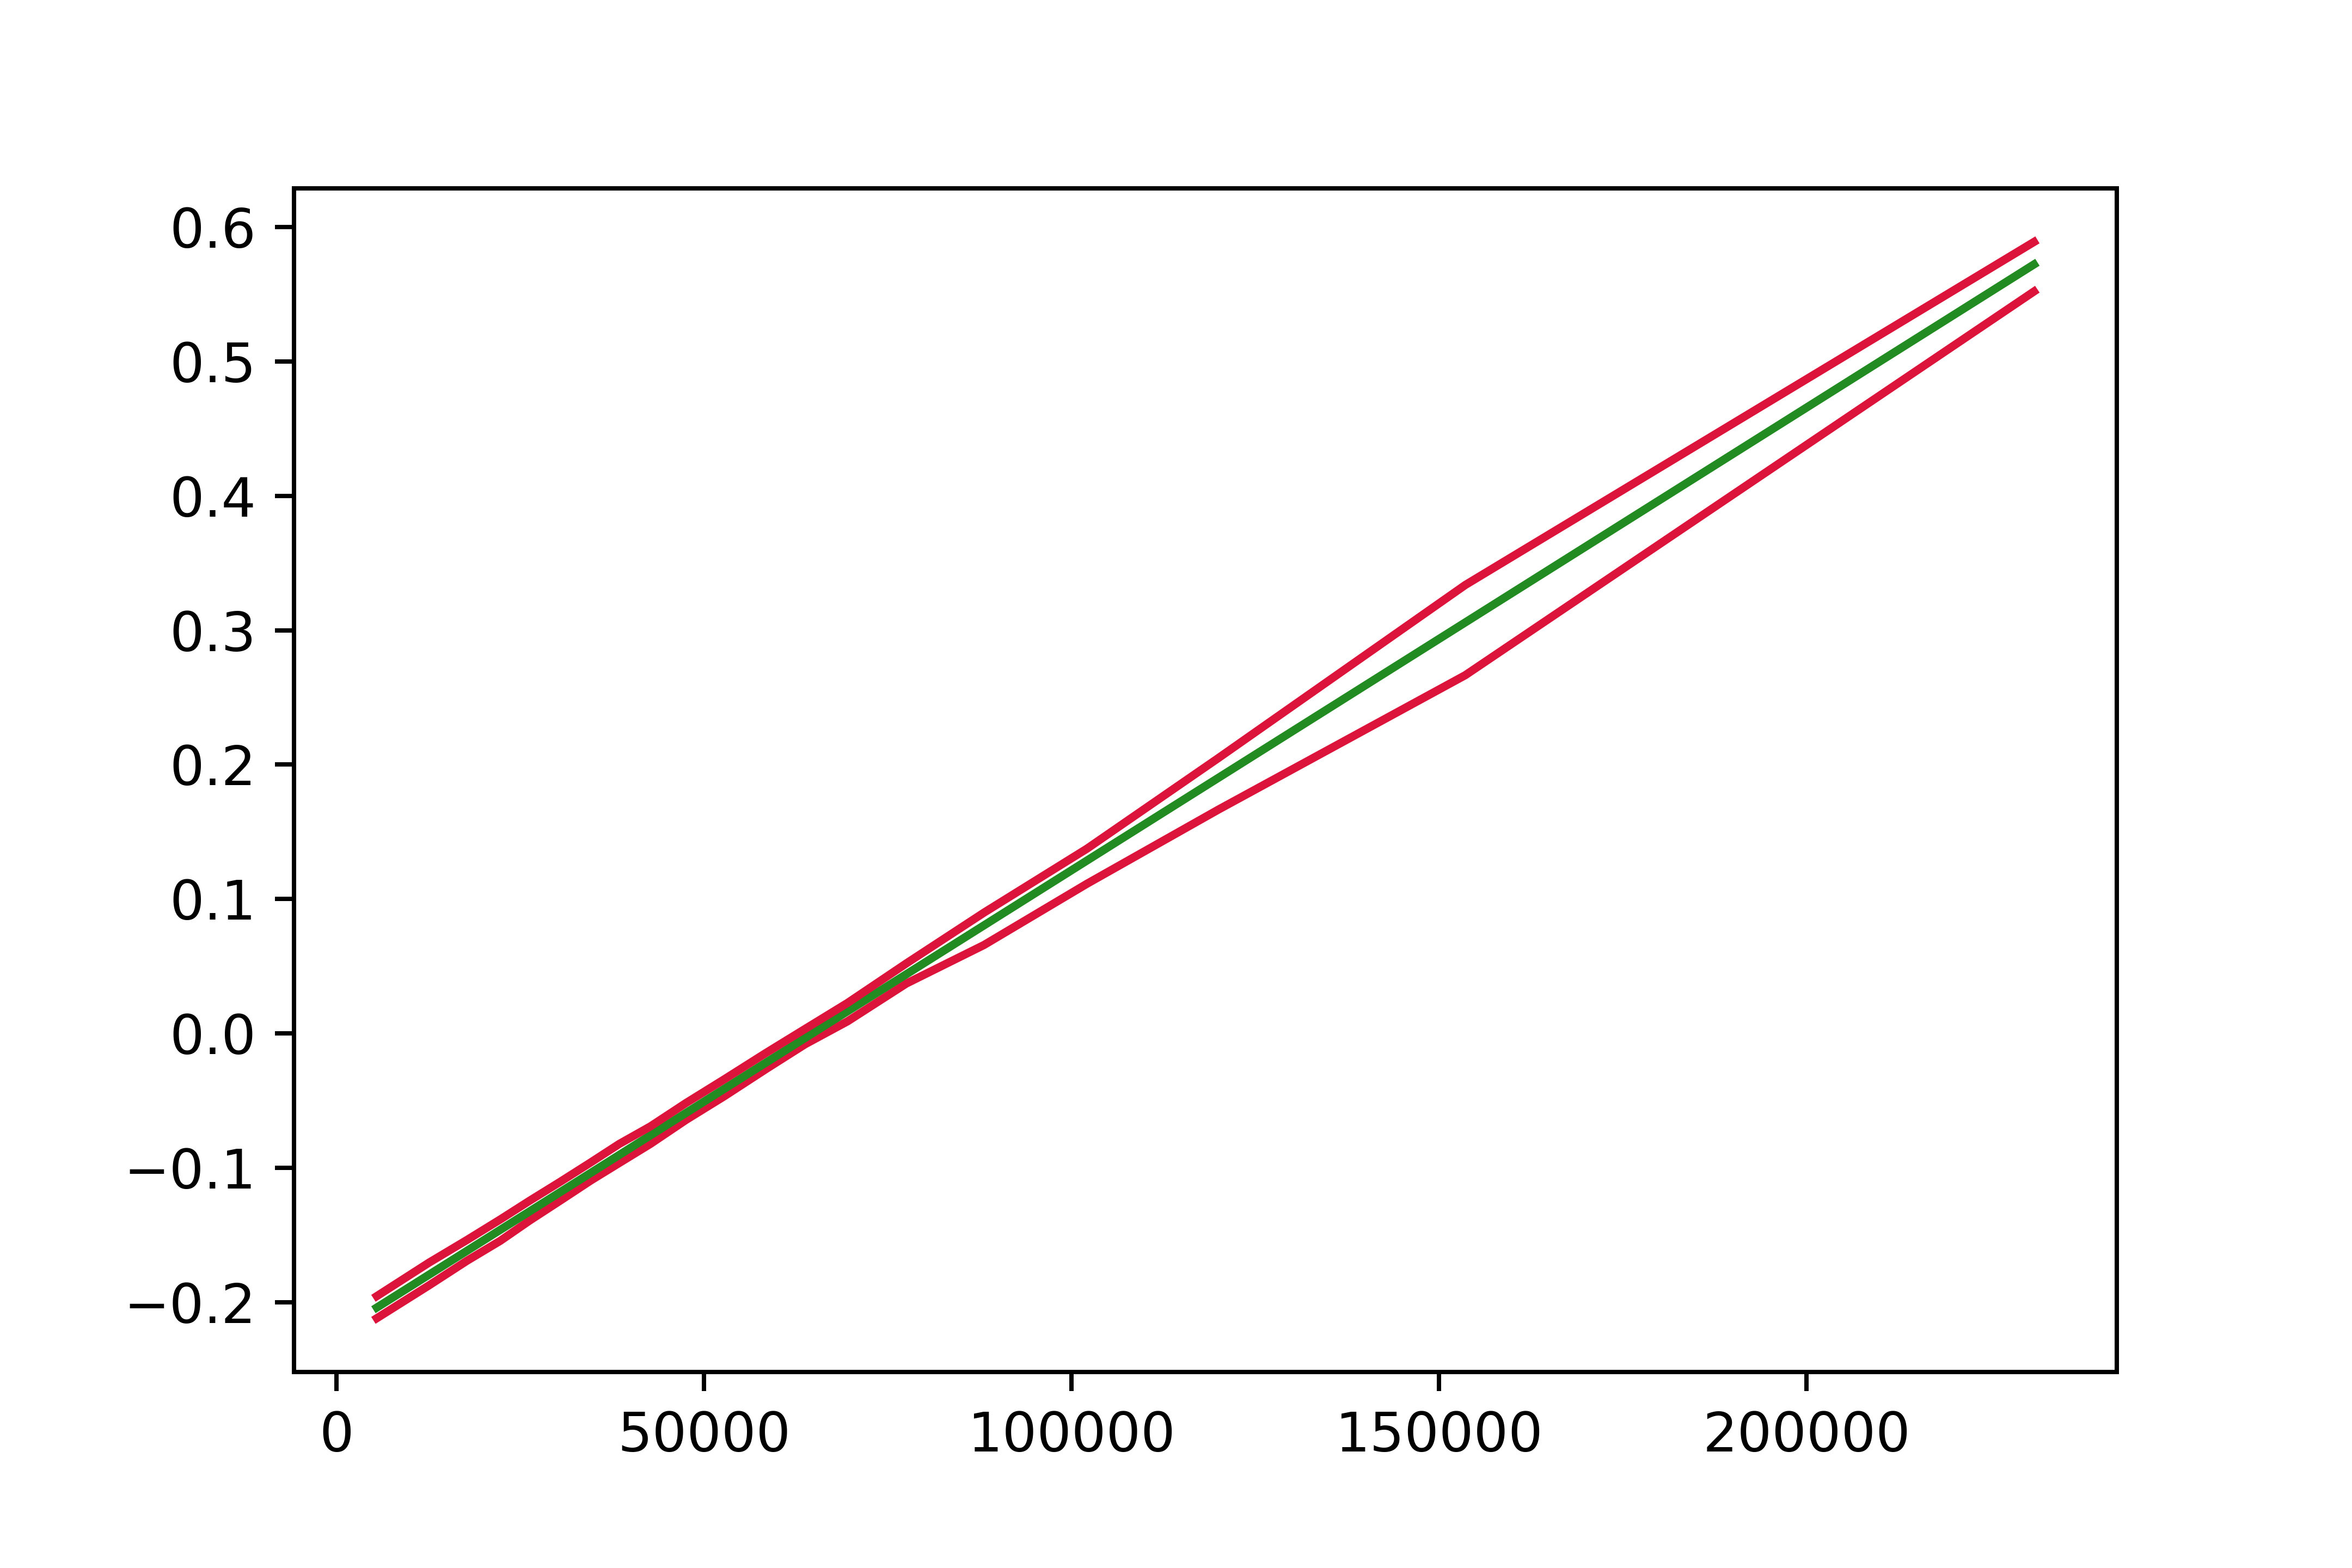
\includegraphics[width=\textwidth]{figures/ALE/chNDexp/spec3_linear_FINCBTXM.png}
        \caption{Income - linear}
    \end{subfigure}\hfill
    \begin{subfigure}{0.5\textwidth}
        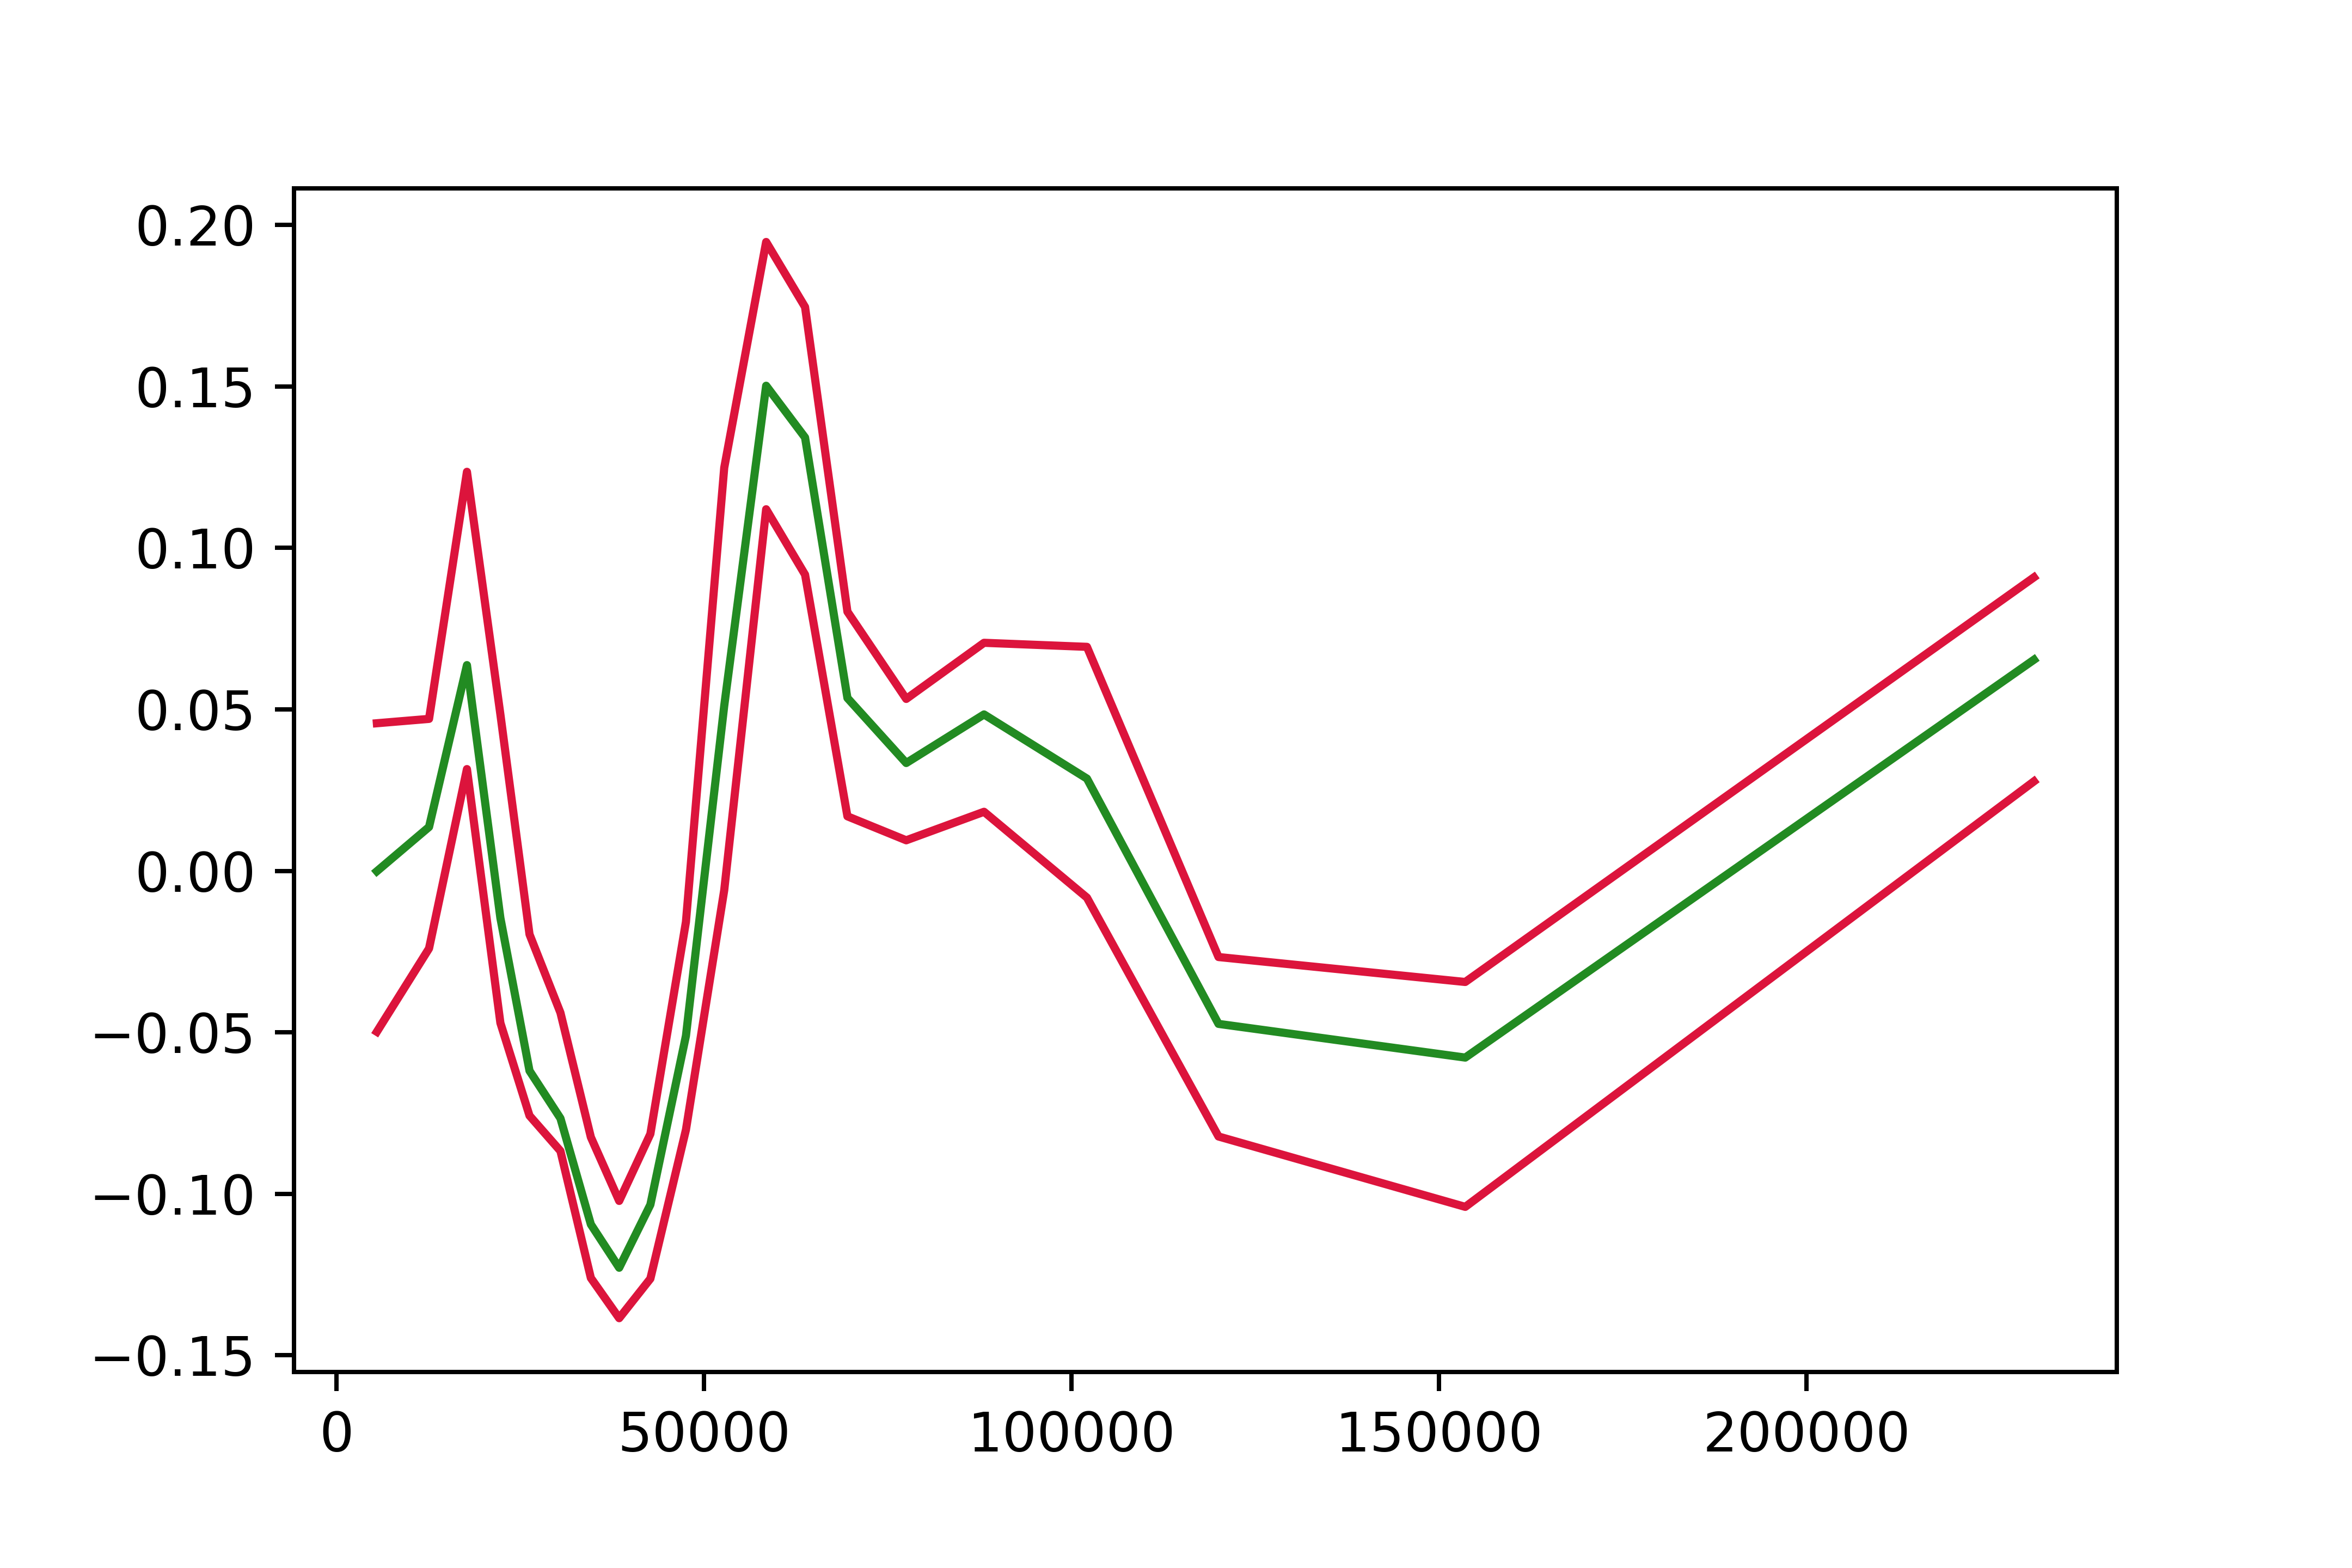
\includegraphics[width=\textwidth]{figures/ALE/chNDexp/spec3_cf_FINCBTXM.png}
        \caption{Income - causal forest}
    \end{subfigure}\hfill
    \caption{ALE of salary and income - non-durable expenditures}
    \label{fig:ale_saleinc}
\end{figure}
Lastly, we turn to the other two financial variables, salary, and income, which are presented in Figure \ref{fig:ale_saleinc}. In both, we see highly non-linear dynamics that appear to be quite similar once a threshold of 50,000 USD is passed. We see that a very low salary leads to a lower MPC, which is reasonable to expect considering the economic circumstances in which the tax rebate took place. Low-income households struggling during the recession might show a smaller response because they use the tax rebate for precautionary savings. On the other hand, the MPC is higher for households that have higher salaries in the range between 50,000 and 75,000 USD before the effect vanishes at higher levels. This is also in line with what we expect as the tax rebate was phased out at reported incomes above 75,000 USD. Thus, high-income households for which the tax rebate plays a minor role in their income anyway received even less. 